\documentclass{beamer}


\usetheme{default}
\usecolortheme{dolphin} 

\usepackage{booktabs} % 用于美化表格
\usepackage{array} % 允许调整列格式

\title{Figures similar to Granja and Paixo Uniform Pricing Paper}
\date{\today}

\begin{document}
\begin{frame}
  \titlepage
\end{frame}

\begin{frame}{Content}
  \tableofcontents
\end{frame}

\section{Overview}
\subsection{About Sample}
\begin{frame}{Overview: About Sample}
    \begin{itemize}
        \item Used the newest RateWatch data, filling in missing values from 2020 to 2021. Covered time range
        \begin{itemize}
            \item from Jan 2015, to Sep 2023, for 12MCD10K, INTCK2.5K, SAV2.5K;
            \item from Jan 2015 to Jun 2022, for SAV25K
        \end{itemize}
        \item According to GP wp, they \textit{“exclude single-branch banks because the aim of our work is to study the pricing policies of banks across their multiple branches.”}
        \begin{itemize}
            \item In multi-branches sample results, we did the same, excluding those ‘inst\_nm’ has only 1 unique ‘accountnumber’, around 7139 observations.
            \item Full sample has 939605 observations, selected sample has 932466 oberservations.
        \end{itemize}
    \end{itemize}
\end{frame}

\subsection{About Figures}
\begin{frame}{Overview: About Figures}
Showing adjusted $R^2$ of interest rates regressed on fixed effects.
    \begin{itemize}
        \item The adjusted $R^2$ are from a monthly series of OLS regressions of interest rates on bank fixed effects, banking market fixed effects, and zip code fixed effects, within each product.
        \item To be more specific, for each month, run an OLS regression of the product rate (observations from branches) on each set of fixed effects, and plot the respective $R^2$ across months.
        \item Skip months with fewer than 10 observations.
    \end{itemize}
\end{frame}


\begin{frame}{Overview: About Figures}
\begin{itemize}

    \item As for the proxies for fixed effects,

\begin{itemize}
        \item Bank fixed effects: ‘primarycompany’ and ‘inst\_nm’;
        \item Zip code fixed effects: the first 3 or 5 or 9 digits of ‘zip’;
        \item Banking market fixed effects: ‘msa’ and ‘cbsa’.
    \end{itemize}

    \item Regarding the coverage scale, empirical evidence suggests that 'cbsa' (clsoe to 'msa') covers a larger area than any digit level of the zip code.
\end{itemize}

\end{frame}

\subsection{About Results}

\begin{frame}{Overview: About Results (Full Sample) }
    \centering
\fontsize{5pt}{6pt}\selectfont
\begin{tabular}{lcccccccc}
    \toprule
    & \textbf{r2\_inst} & \textbf{r2\_primarycompany} & \textbf{r2\_zip9} & \textbf{r2\_zip5} & \textbf{r2\_zip3} & \textbf{r2\_msa} & \textbf{r2\_cbsa} & \textbf{r2\_county} \\
    \midrule
    12MCD10K   & 0.9117 & 0.8145 & 0.7908 & 0.6633 & 0.3864 & 0.1757 & 0.2889 & 0.3751 \\
    INTCK2.5K  & 0.8221 & 0.7539 & 0.8810 & 0.6846 & 0.5435 & 0.2223 & 0.2583 & 0.4501 \\
    SAV2.5K    & 0.9358 & 0.9331 & 0.7635 & 0.6861 & 0.4030 & 0.1305 & 0.2992 & 0.4527 \\
    SAV25K     & 0.9633 & 0.9622 & 0.8422 & 0.7822 & 0.4308 & 0.2674 & 0.3406 & 0.4120 \\
    \midrule
    \textbf{AVG} & 0.9083 & 0.8659 & 0.8194 & 0.7041 & 0.4409 & 0.1990 & 0.2968 & 0.4225 \\
    \bottomrule
\end{tabular}

\end{frame}


\begin{frame}{Overview: About Results (Multi-branches Sample) }

    \centering
\fontsize{5pt}{6pt}\selectfont
        \begin{tabular}{lcccccccc}
        \toprule
        & \textbf{r2\_inst} & \textbf{r2\_primarycompany} & \textbf{r2\_zip9} & \textbf{r2\_zip5} & \textbf{r2\_zip3} & \textbf{r2\_msa} & \textbf{r2\_cbsa} & \textbf{r2\_county} \\
        \midrule
        12MCD10K   & 0.8716 & 0.7334 & 0.8765 & 0.6817 & 0.4555 & 0.2040 & 0.2510 & 0.3596 \\
        INTCK2.5K  & 0.8226 & 0.7608 & 0.8812 & 0.6840 & 0.5431 & 0.2221 & 0.2586 & 0.4484 \\
        SAV2.5K    & 0.8372 & 0.8303 & 0.8889 & 0.7397 & 0.5884 & 0.1468 & 0.1657 & 0.4260 \\
        SAV25K     & 0.8911 & 0.8854 & 0.9768 & 0.8064 & 0.5741 & 0.3039 & 0.3077 & 0.4538 \\
        \midrule
        \textbf{AVG} & 0.8556 & 0.8025 & 0.9059 & 0.7280 & 0.5403 & 0.2192 & 0.2457 & 0.4219 \\
        \bottomrule
    \end{tabular}
\end{frame}



\begin{frame}{Overview: About Results}
\begin{enumerate}
    \item Generally, the results show that bank fixed effects account for the most variance, followed by zip code fixed effects, while banking market fixed effects contribute the least.
    \item For bank fixed effects, 'inst\_nm' accounts for more variance than 'primarycompany', indicating that \textbf{pricing is more unified within a specific secondary institution of a bank.}
    \item For zip code fixed effects, as the area scale increases from 9 digits to 3 digits, the variance explained decreases.
    \item A similar pattern is observed when comparing banking market and zip code effects, since CBSA or MSA includes multiple zip codes.
\end{enumerate}
\end{frame}

\subsection{About Questions}

\begin{frame}{Overview: About Questions}
\begin{enumerate}
        \item According to GP wp, zip code fixed effects account for, on average, less than 30\% of the total variance in interest rates within the banking sector. \\
        Our results strongly suggest that they might have used the 3 digits zip code.
        
        \item When selecting the sample, the conclusion appears to be a bit less robust, and more random.\\
        The SAV25K is the least robust, while the INTCK2.5K displays some unusual periods (Dec 2018 to Aug 2019).
        
        \item There is no clear explanation of the proxy GP used for the "banking market." \\ 
        If the proxy is MSA, CBSA, or county, it covers a larger geographic area than a zip code. Shouldn’t zip codes then explain more variance than the banking market? In GP wp, they account for less.
    \end{enumerate}

\end{frame}


% Brief description and charts
\section{Run Reg on the Full Sample}

\subsection{The 3 Fixed Effects Proxies (similar to GP wp)}

\begin{frame}
    \vfill
    \centering
    {\usebeamercolor[fg]{structure} Full sample, figures similar to GP wp,}
    
    \begin{enumerate}
        \item Showing adjusted $R^2$ of rate regress on the following fixed effects, 
            
            Bank (inst\_nm), Zip Code (3 digits), Banking Market (MSA)
        \item Regression on the full sample, {\textbf{\usebeamercolor[fg]{structure}including}} 'inst\_nm's that have only single 'accountnumber'
    \end{enumerate}
    \vfill
\end{frame}

\begin{frame}{12MCD0K, full sample}
\begin{center}
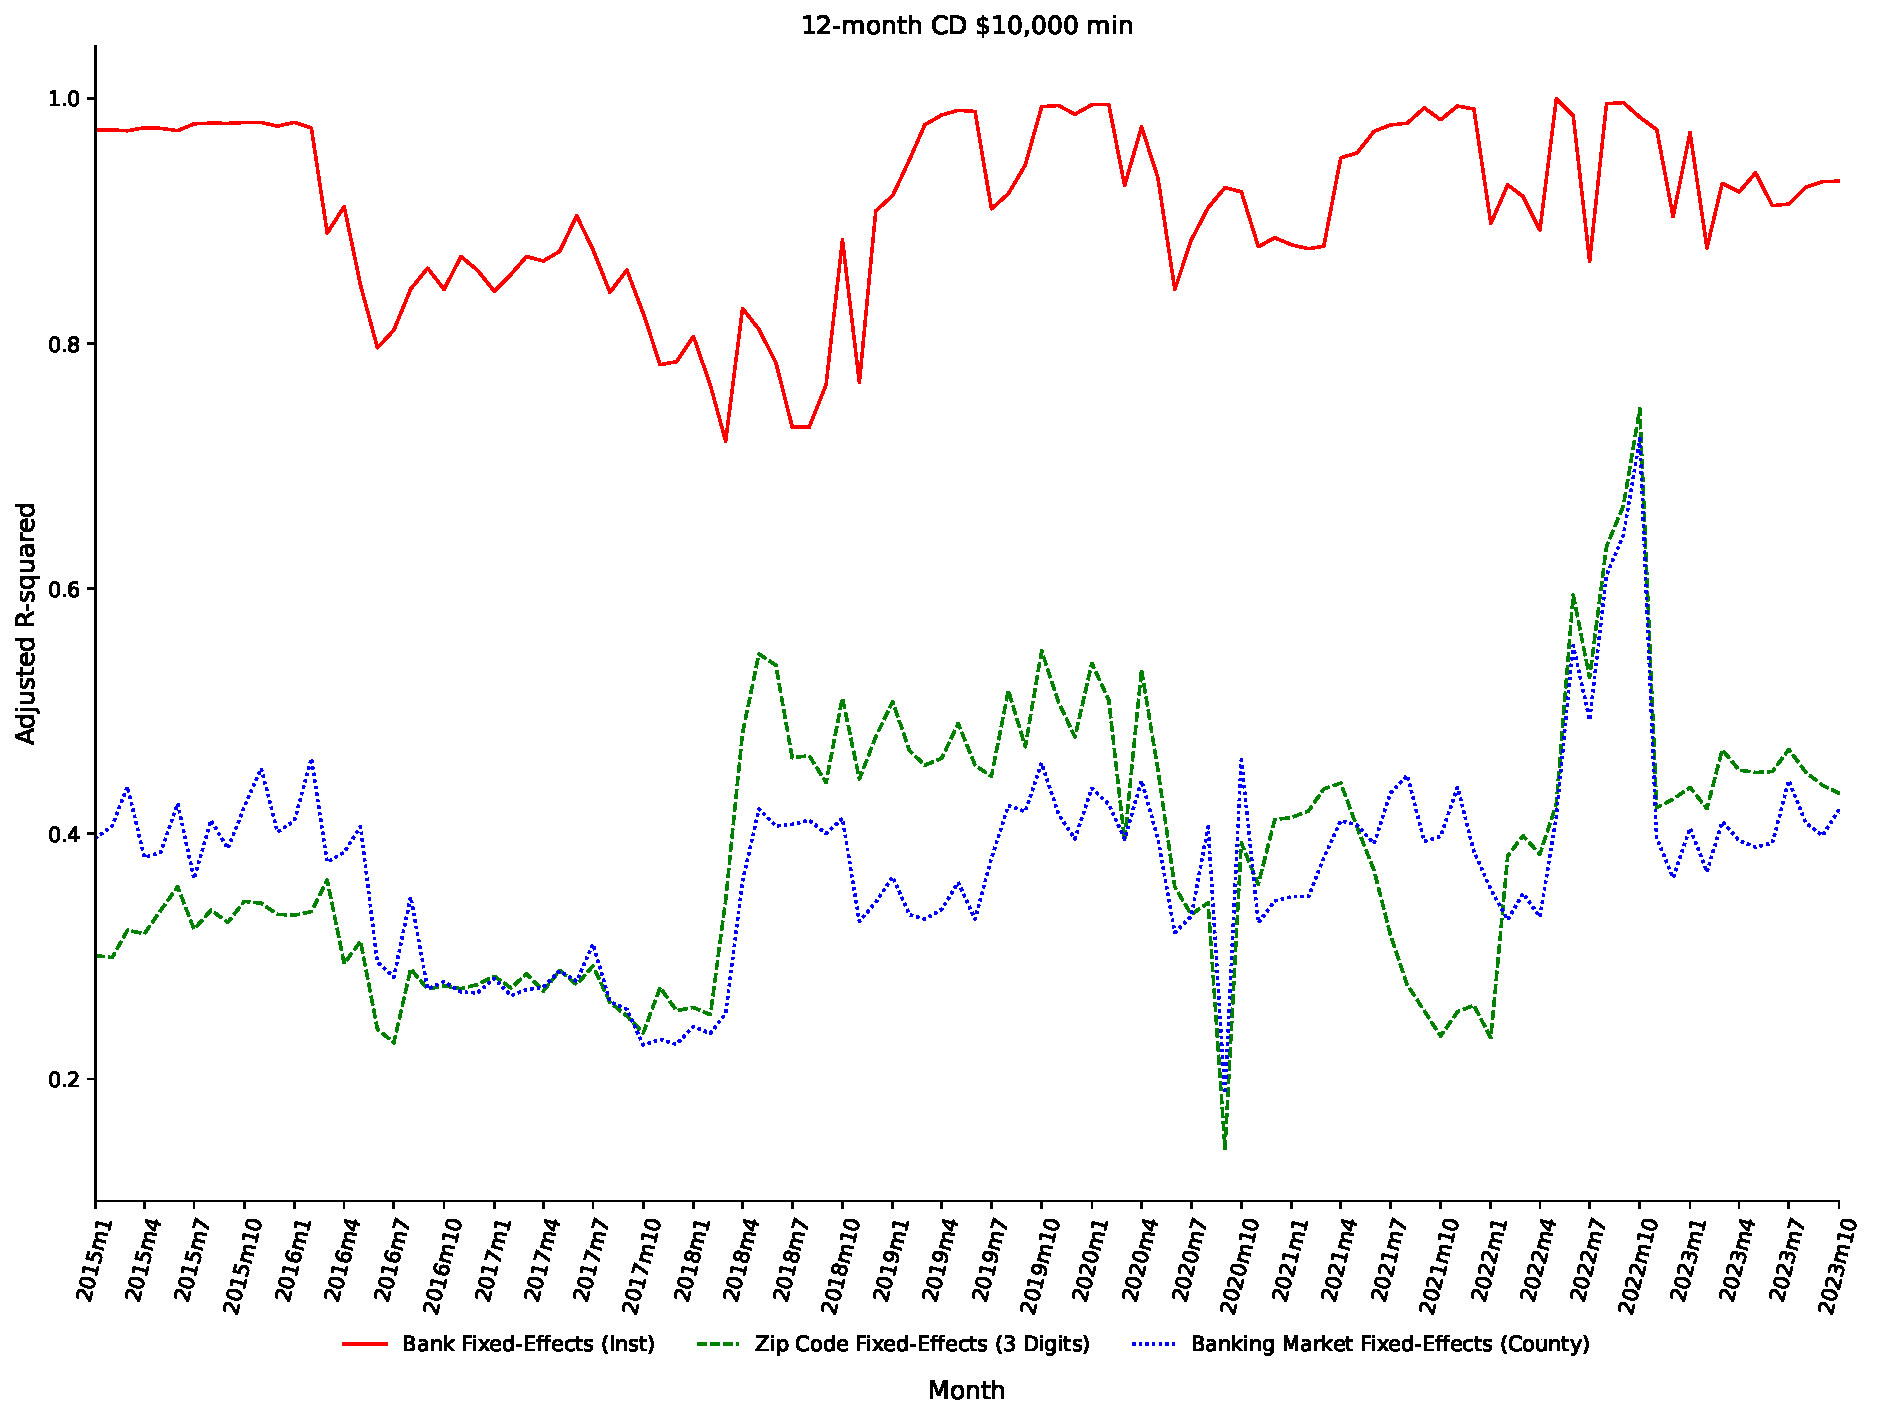
\includegraphics[width=1\textwidth]{figure/all_sample_939605/3_fixed_effects_same_as_GP_wp/12MCD10K_adjusted_R2_Rate_3_fixed_effects.pdf} 
\end{center}
\end{frame}


\begin{frame}{INTCK2.5K, full sample}
\begin{center}
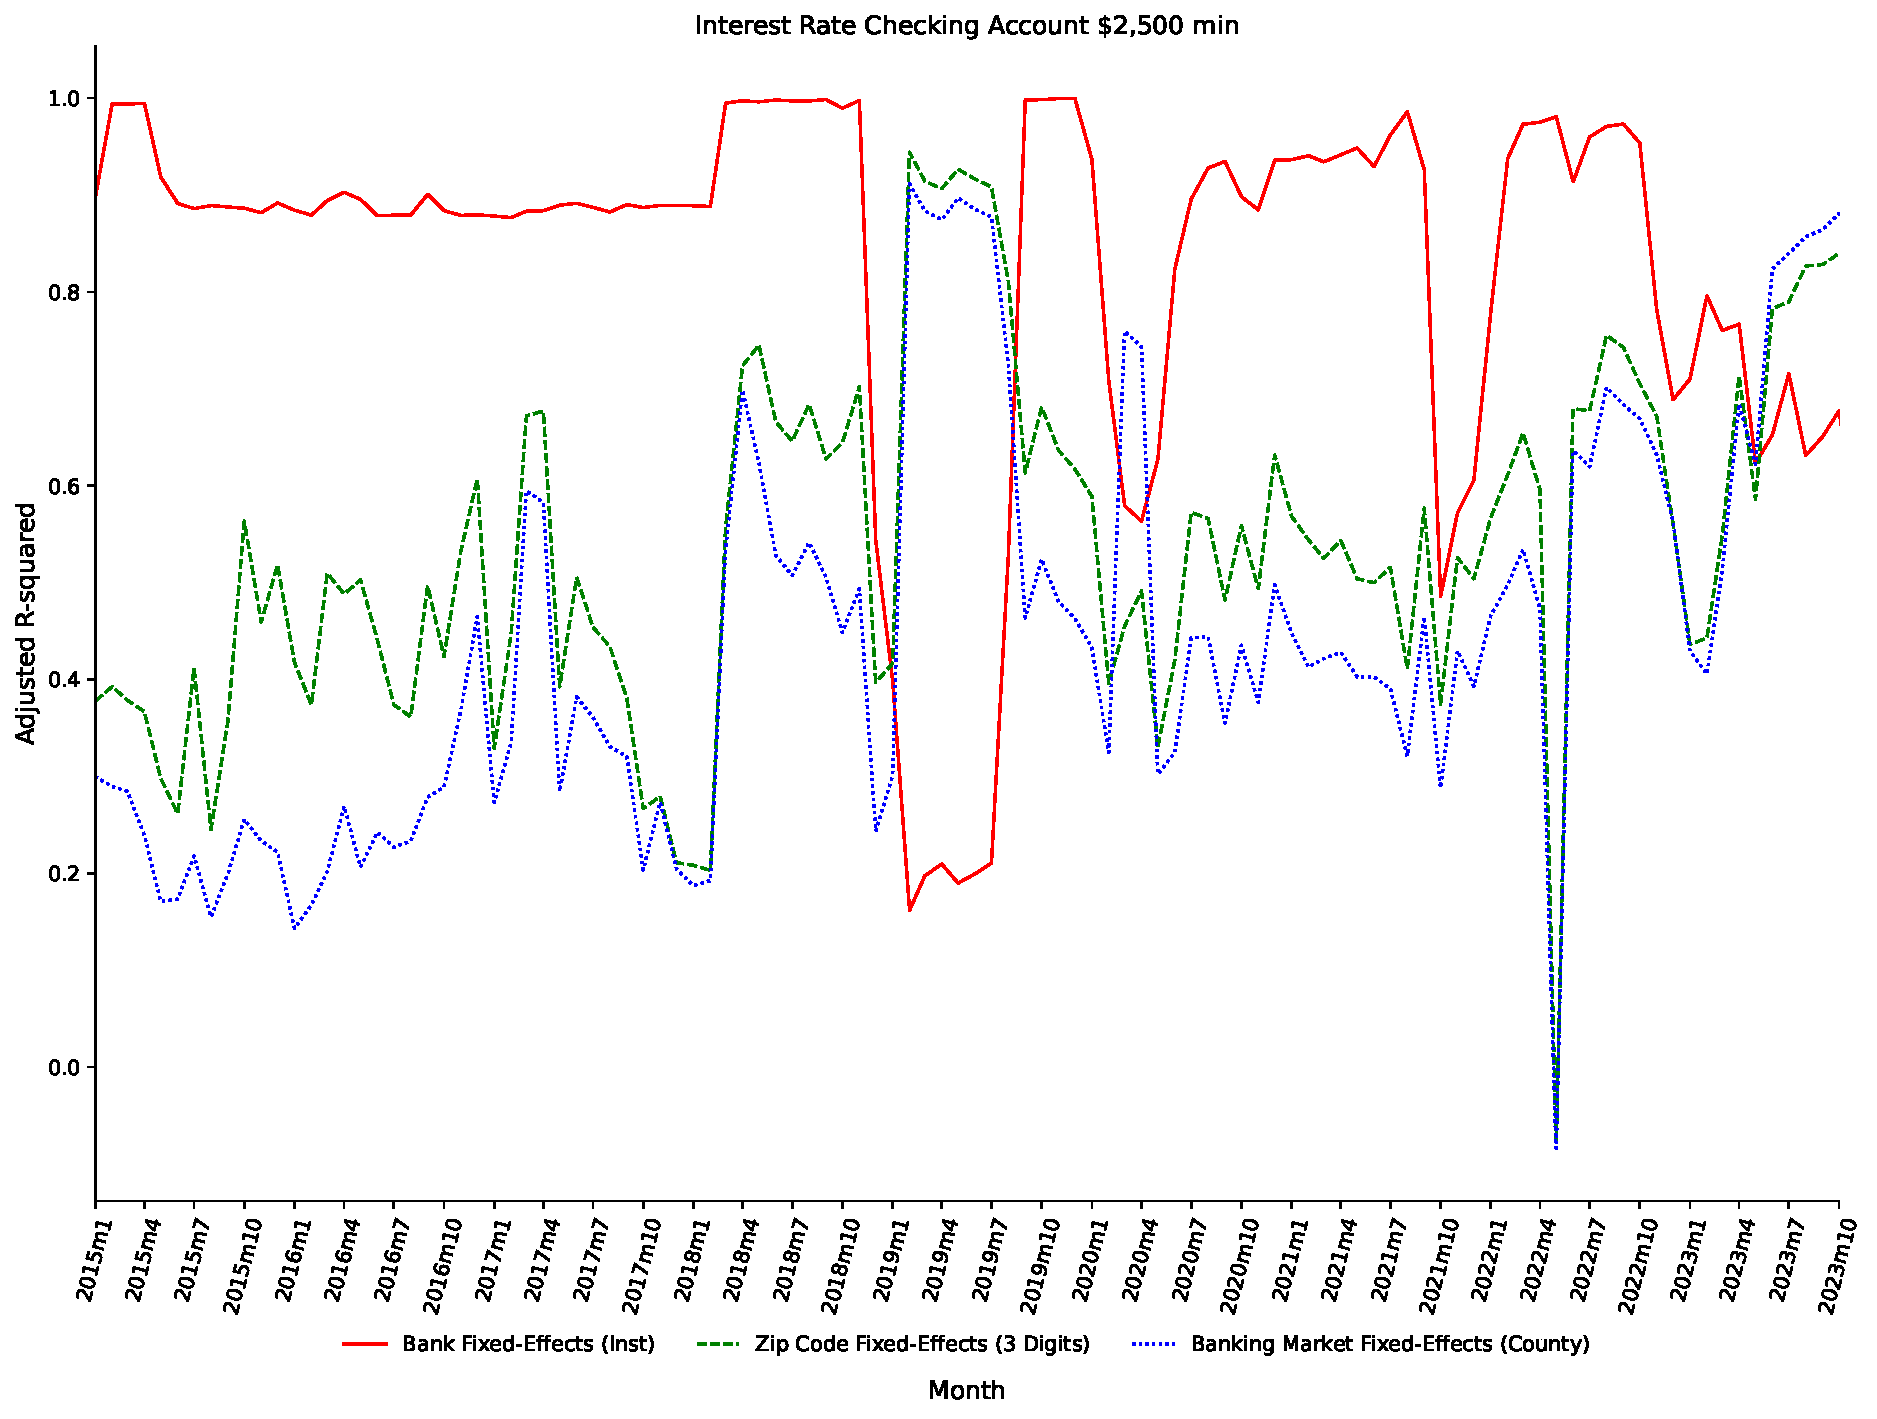
\includegraphics[width=1\textwidth]{figure/all_sample_939605/3_fixed_effects_same_as_GP_wp/INTCK2_5K_adjusted_R2_Rate_3_fixed_effects.pdf} 
\end{center}
\end{frame}



\begin{frame}{SAV2.5K, full sample}
\begin{center}
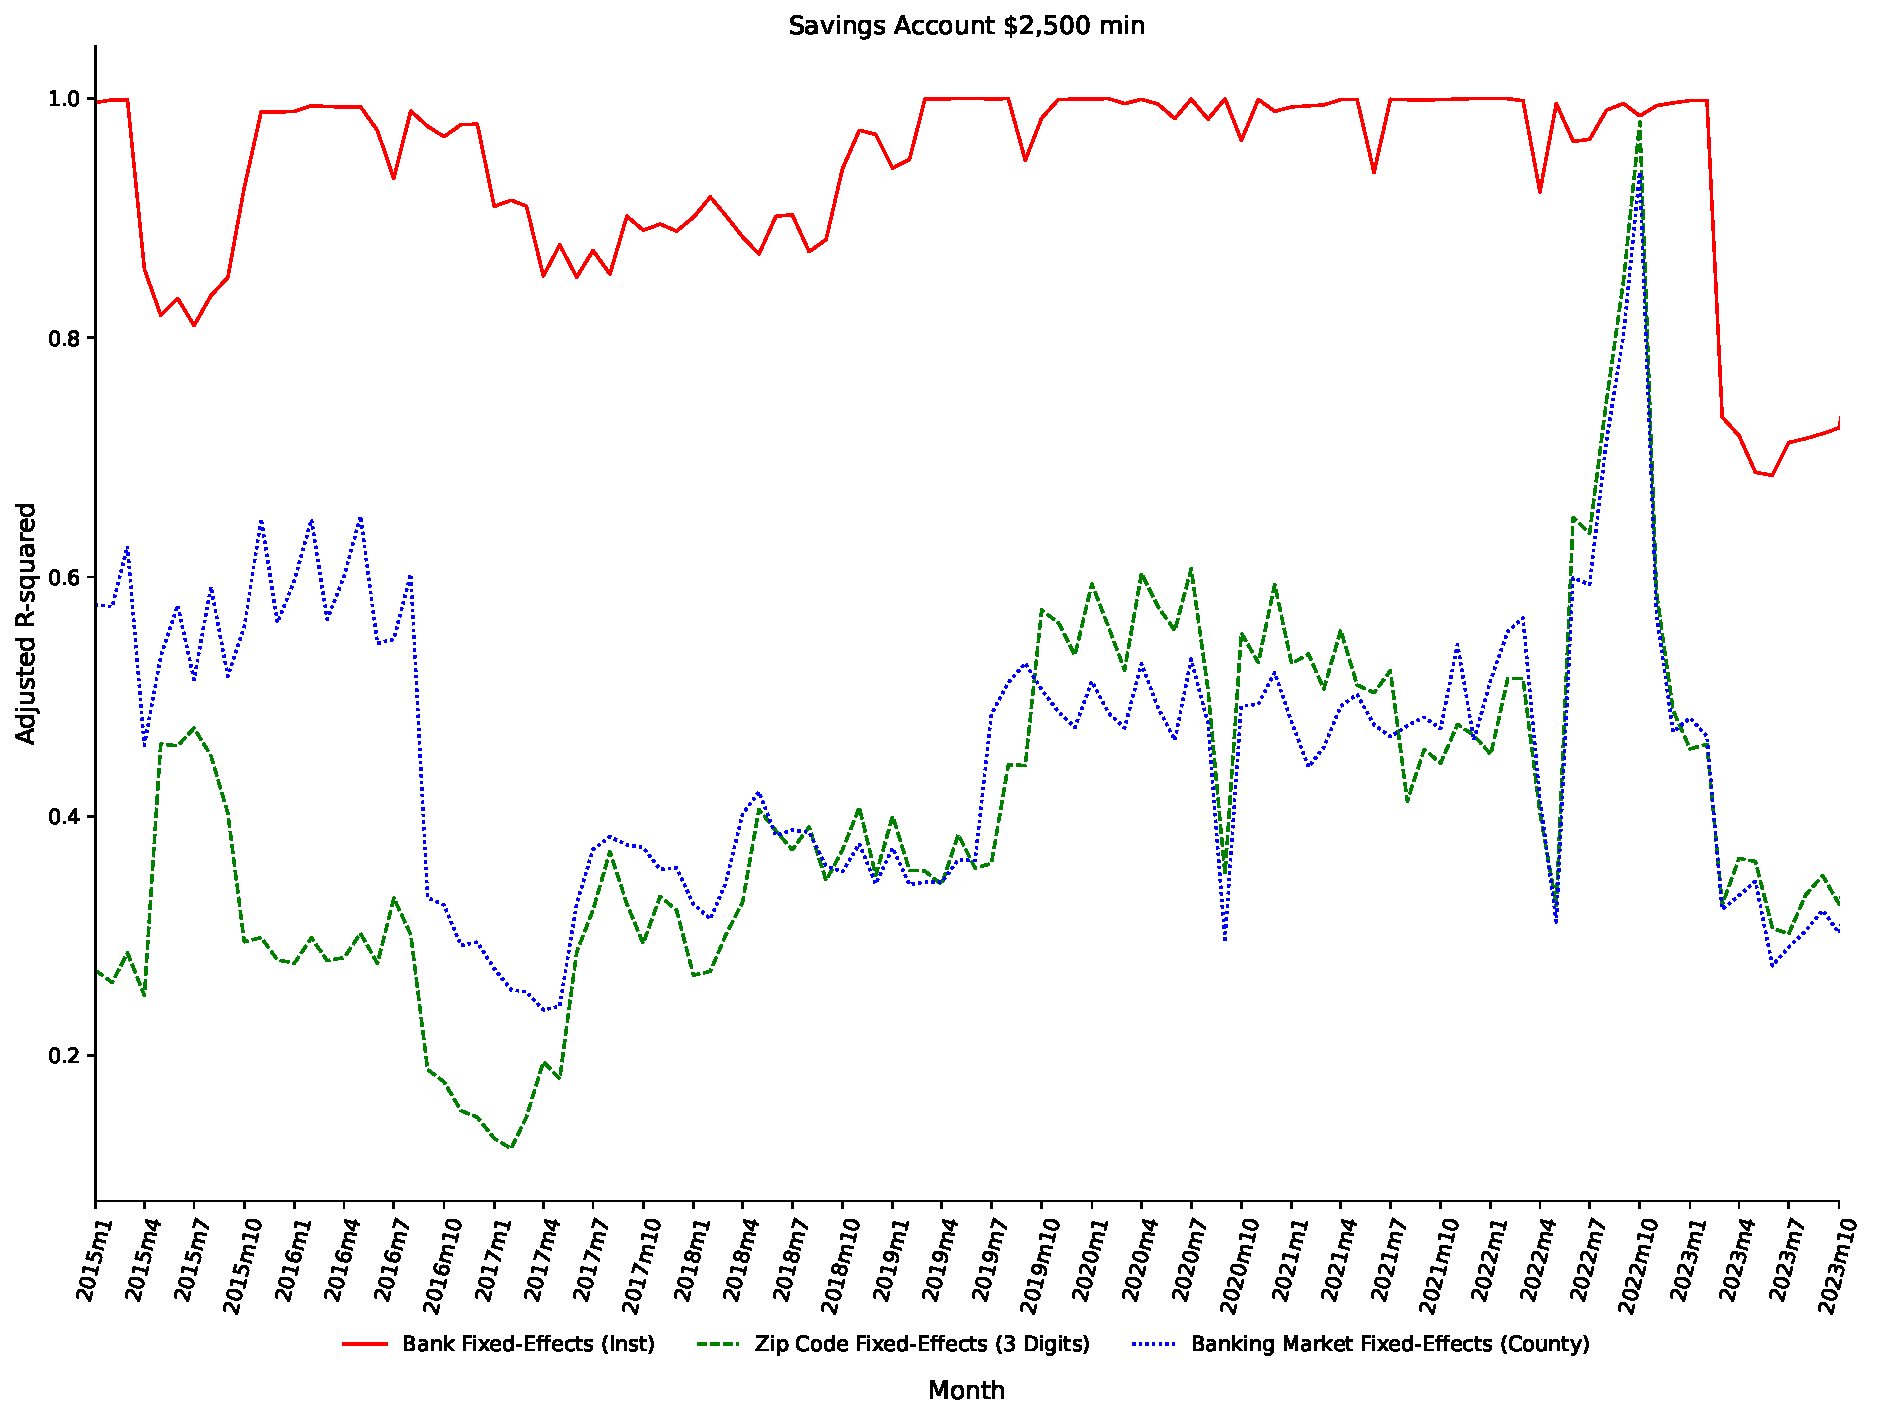
\includegraphics[width=1\textwidth]{figure/all_sample_939605/3_fixed_effects_same_as_GP_wp/SAV2_5K_adjusted_R2_Rate_3_fixed_effects.pdf} 
\end{center}
\end{frame}



\begin{frame}{SAV25K, full sample}
\begin{center}
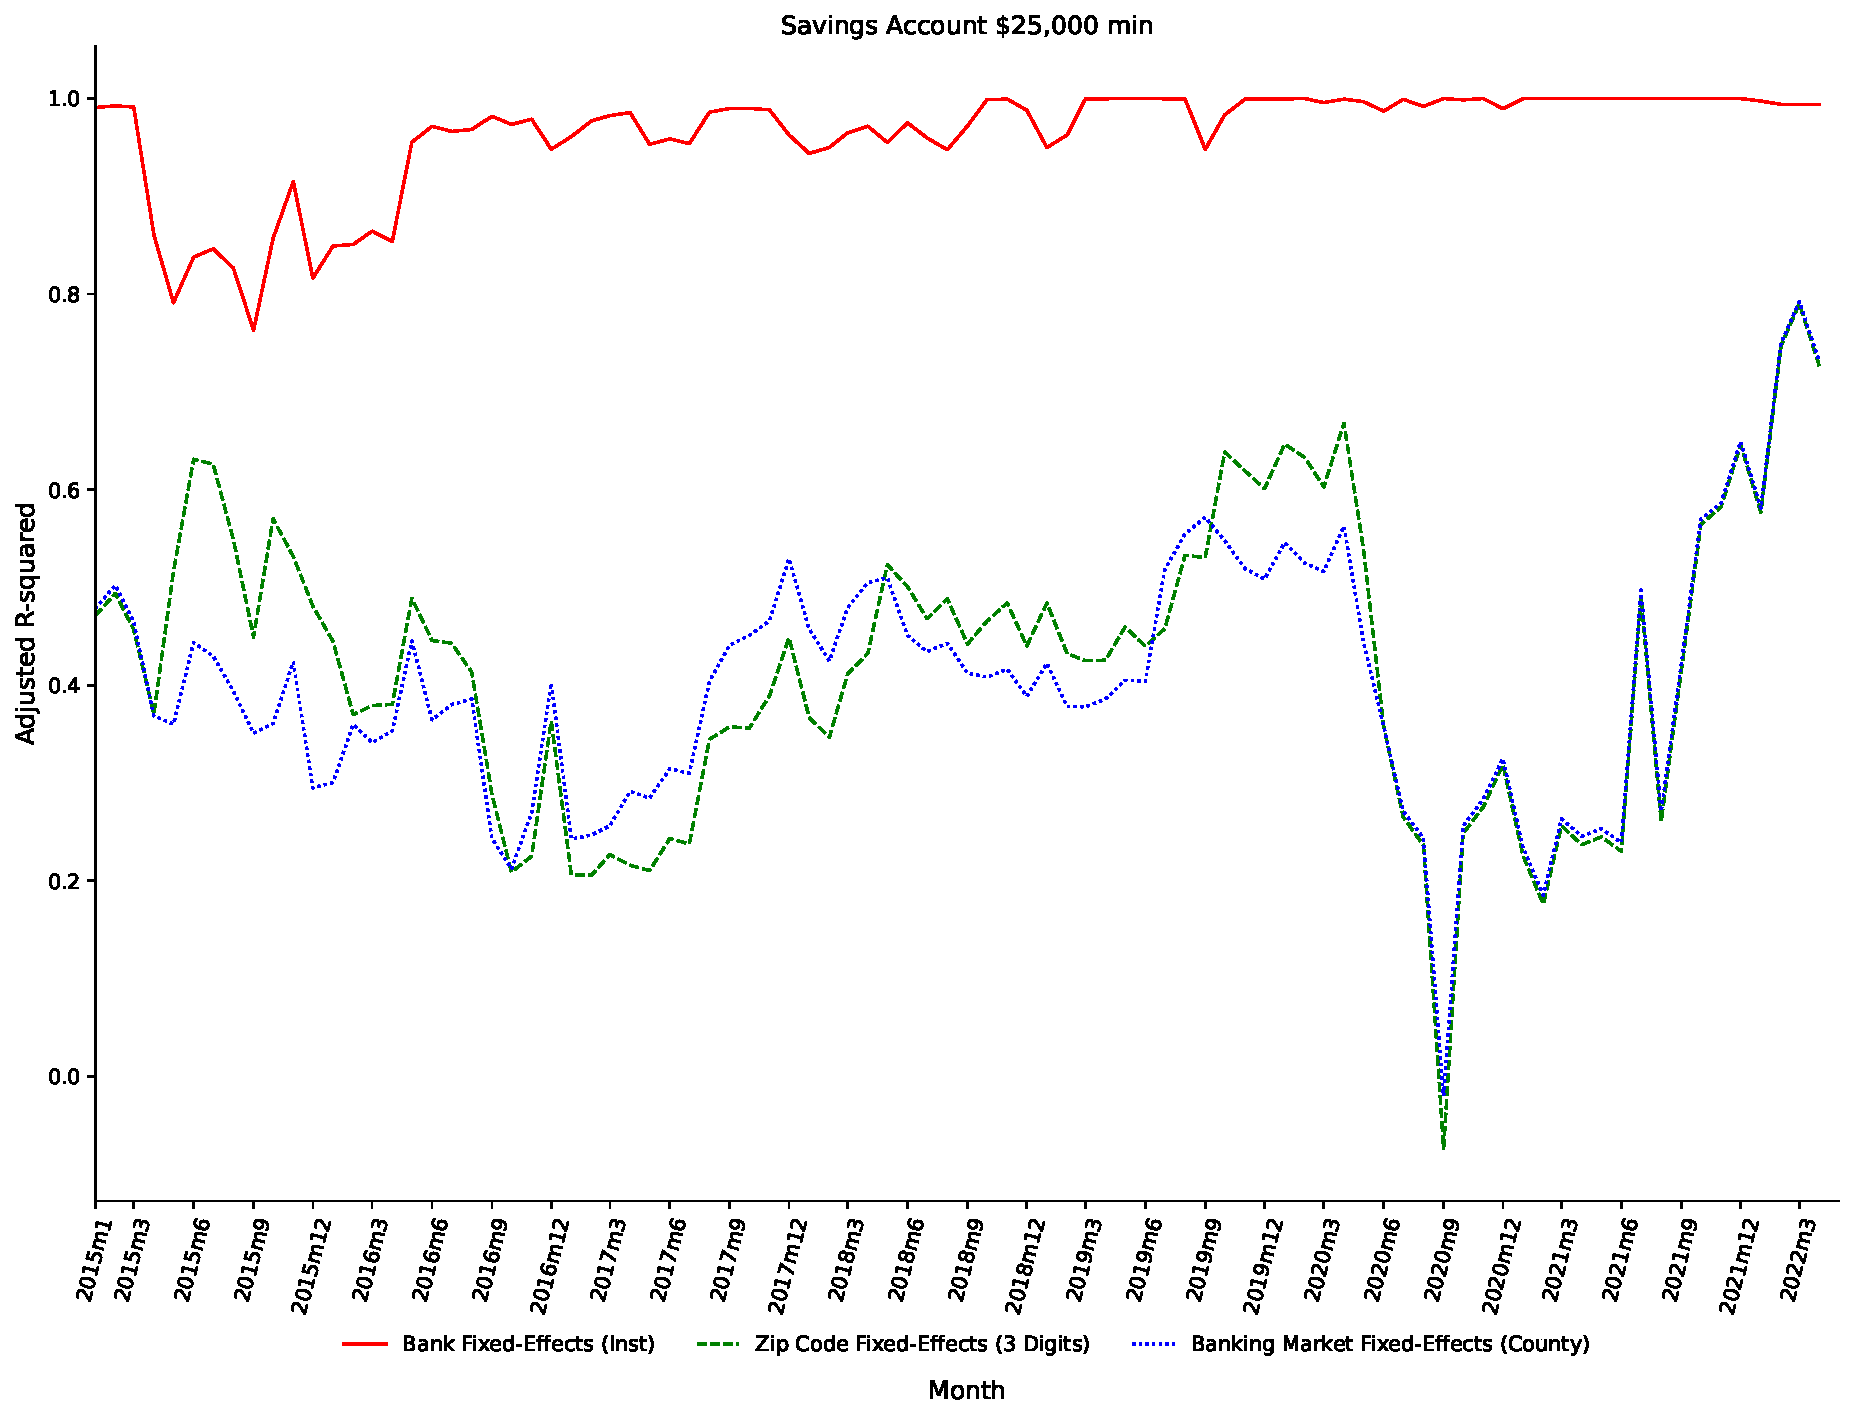
\includegraphics[width=1\textwidth]{figure/all_sample_939605/3_fixed_effects_same_as_GP_wp/SAV25K_adjusted_R2_Rate_3_fixed_effects.pdf} 
\end{center}
\end{frame}


\subsection{Comparison of all fixed effects proxies}

\begin{frame}
    \vfill
    \centering
    {\usebeamercolor[fg]{structure}Full sample, figures comparing all possible proxies,}
    \begin{enumerate}
        \item Showing adjusted $R^2$ of rate regress on fixed effects, using the following proxies, 
        \begin{itemize}
            \item Bank fixed effects: 'primarycompany' and 'inst\_nm
            \item Banking market fixed effects: 'msa' and 'cbsa'
            \item Zip code fixed effects: the first 3 or 5 or 9 digits of 'zip'
        \end{itemize}    
        \item Regression on the full sample, {\textbf{\usebeamercolor[fg]{structure}including}} 'inst\_nm's that have only single 'accountnumber'
    \end{enumerate}
    \vfill
\end{frame}



\begin{frame}{12MCD0K, full sample}
\begin{center}
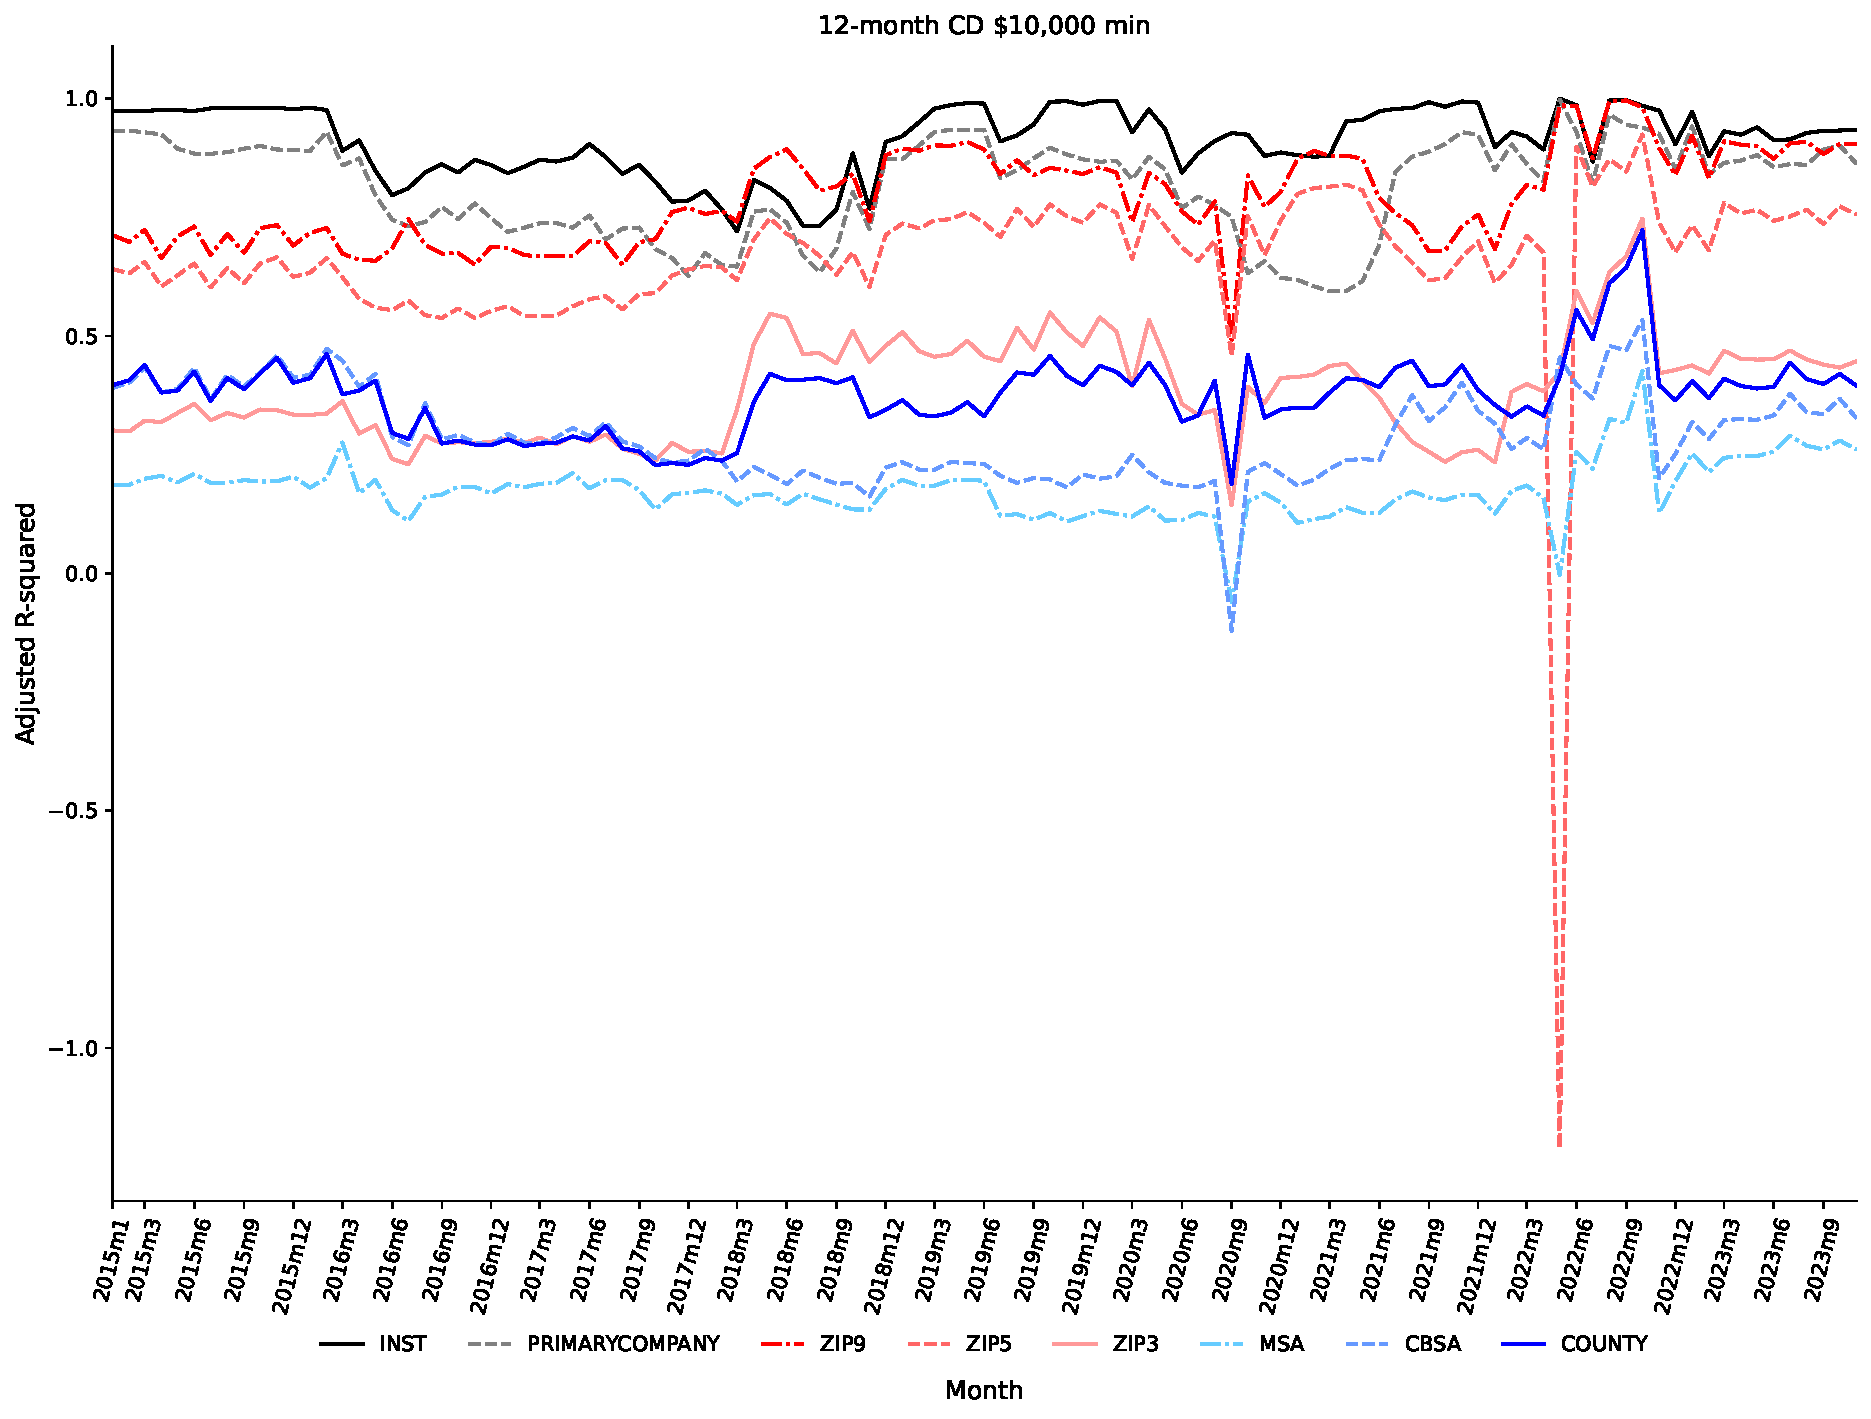
\includegraphics[width=1\textwidth]{figure/all_sample_939605/all_fixed_effects/12MCD10K_adjusted_R2_all_fixed_effects.pdf} 
\end{center}
\end{frame}


\begin{frame}{INTCK2.5K, full sample}
\begin{center}
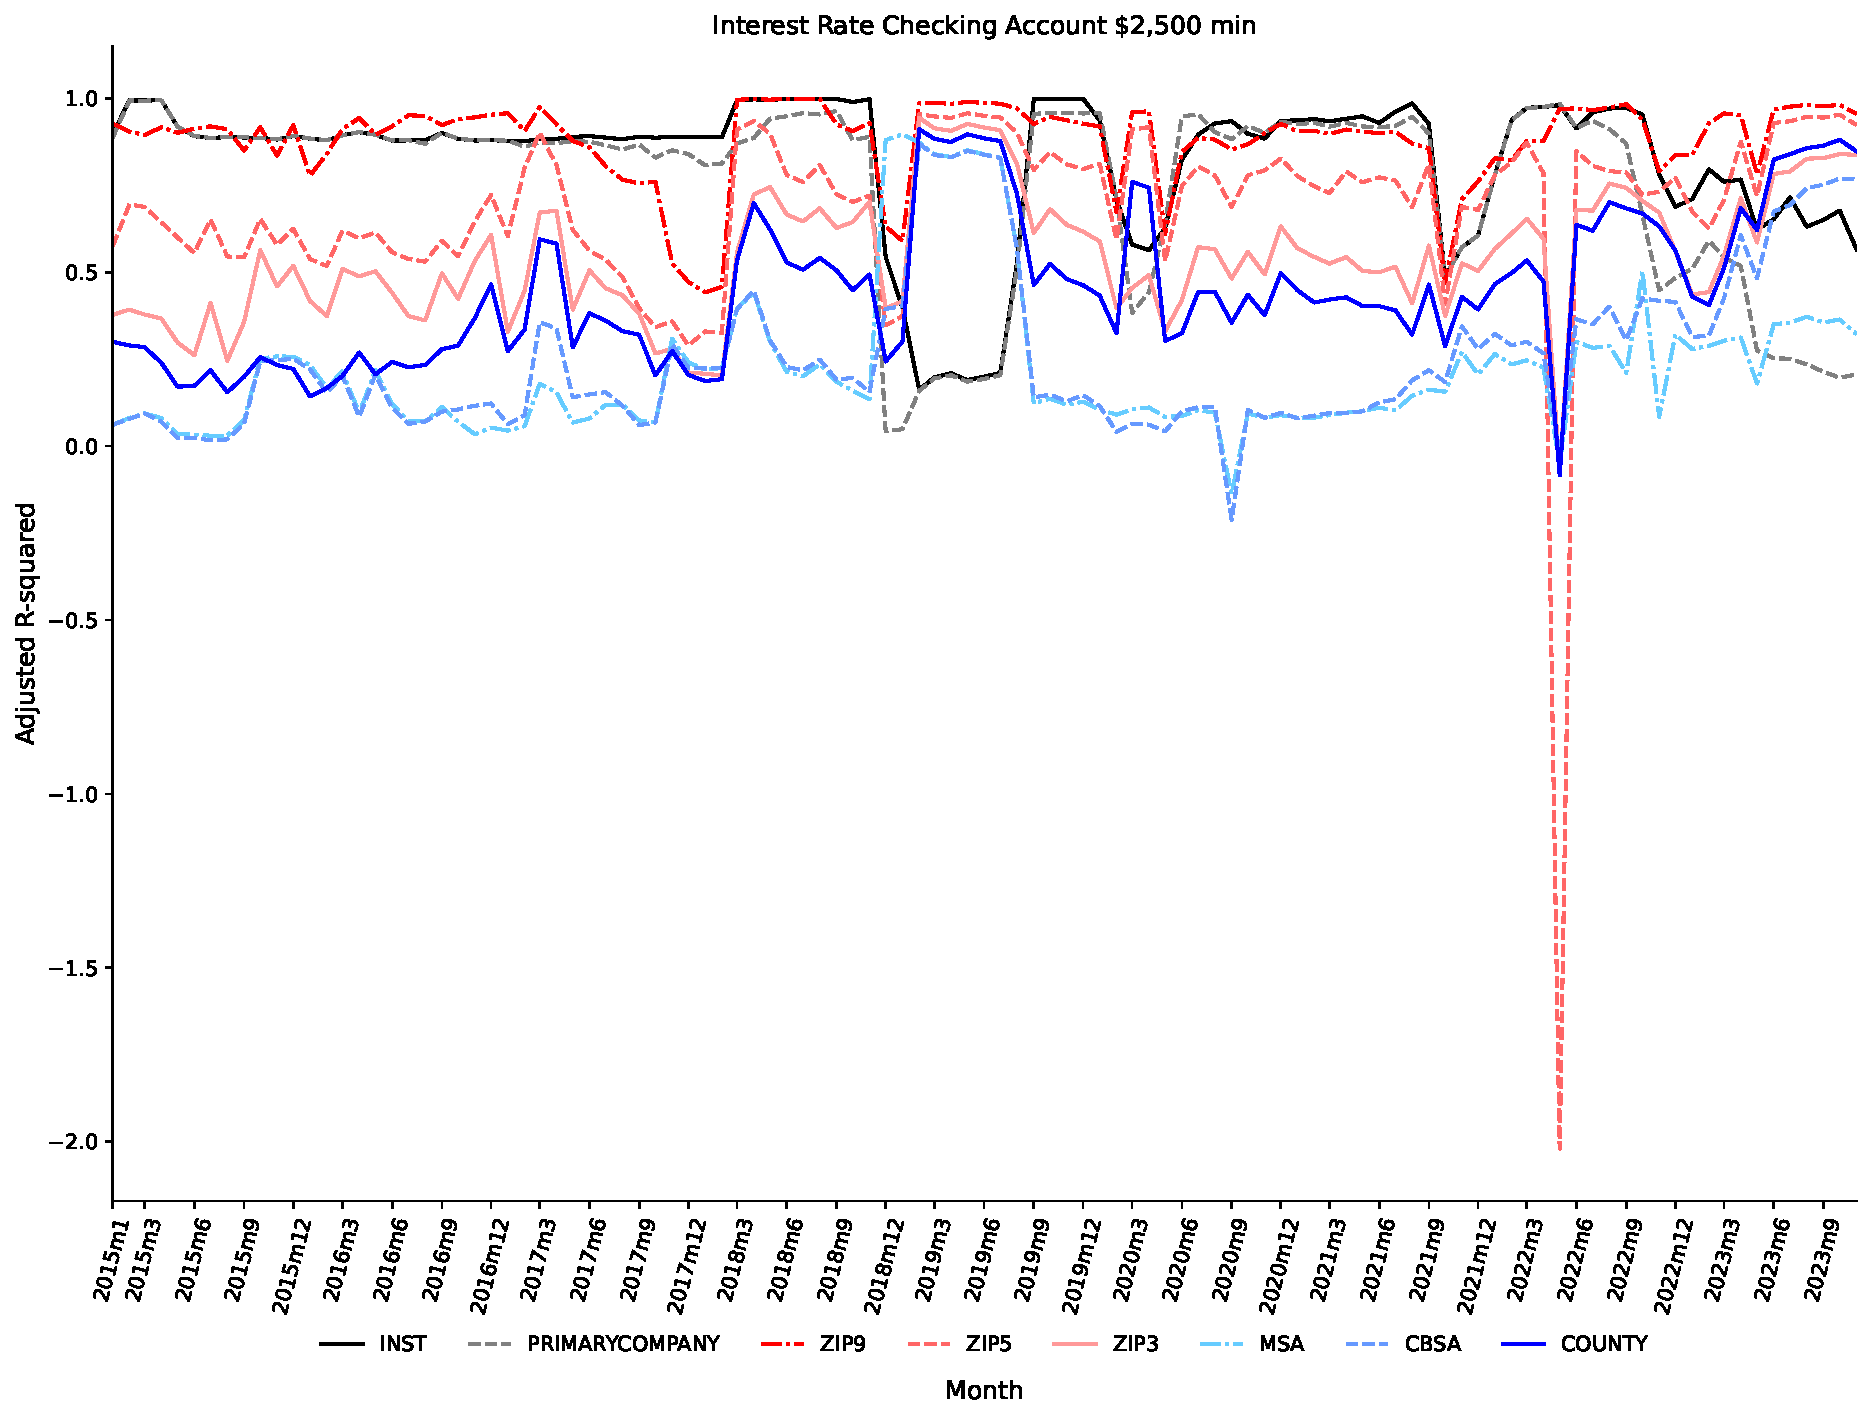
\includegraphics[width=1\textwidth]{figure/all_sample_939605/all_fixed_effects/INTCK2_5K_adjusted_R2_all_fixed_effects.pdf} 
\end{center}
\end{frame}



\begin{frame}{SAV2.5K, full sample}
\begin{center}
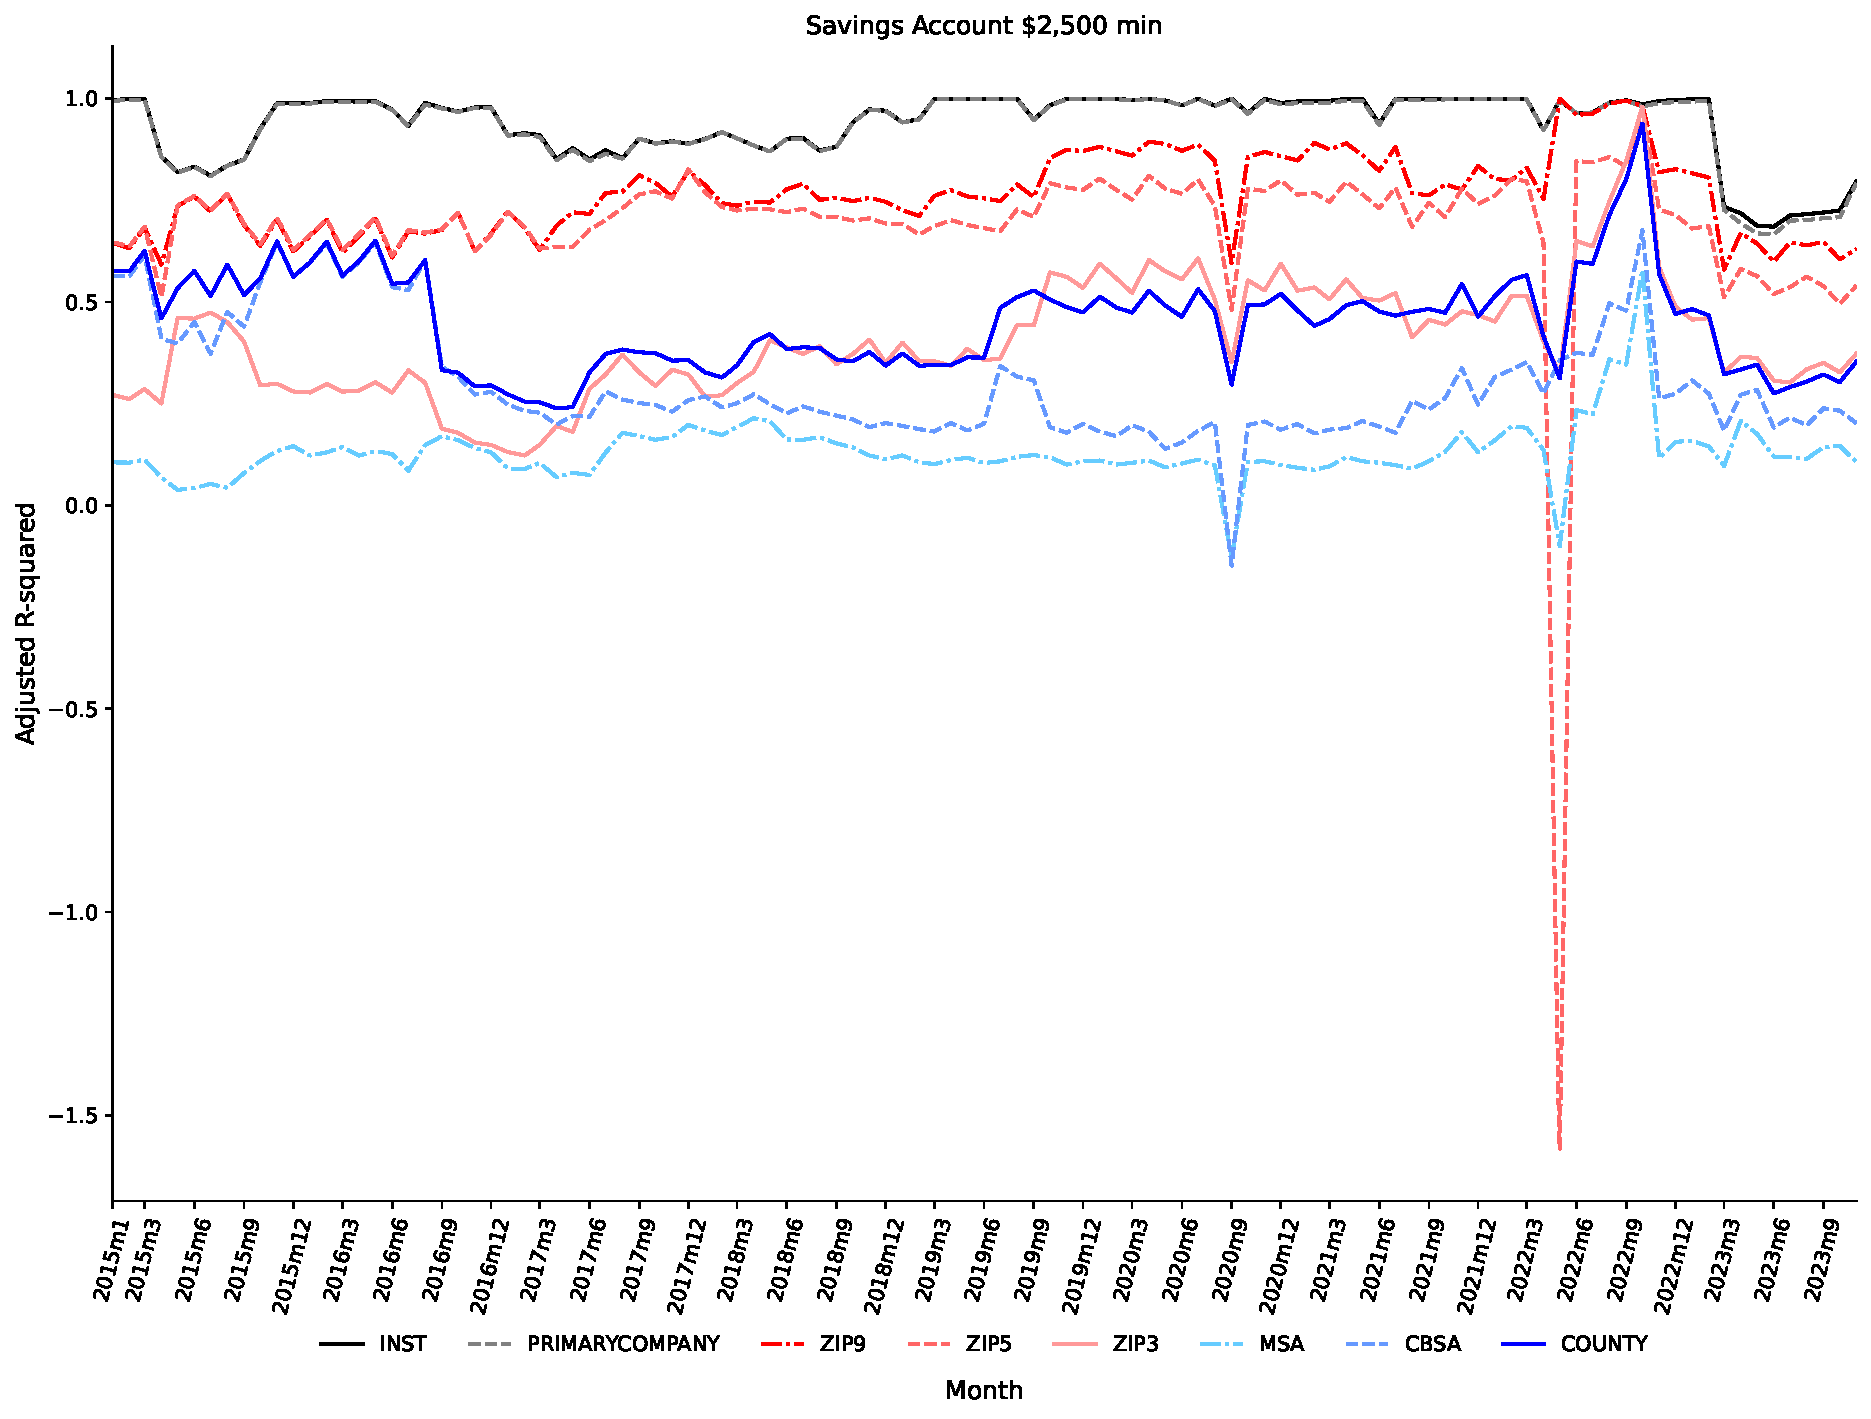
\includegraphics[width=1\textwidth]{figure/all_sample_939605/all_fixed_effects/SAV2_5K_adjusted_R2_all_fixed_effects.pdf} 
\end{center}
\end{frame}



\begin{frame}{SAV25K, full sample}
\begin{center}
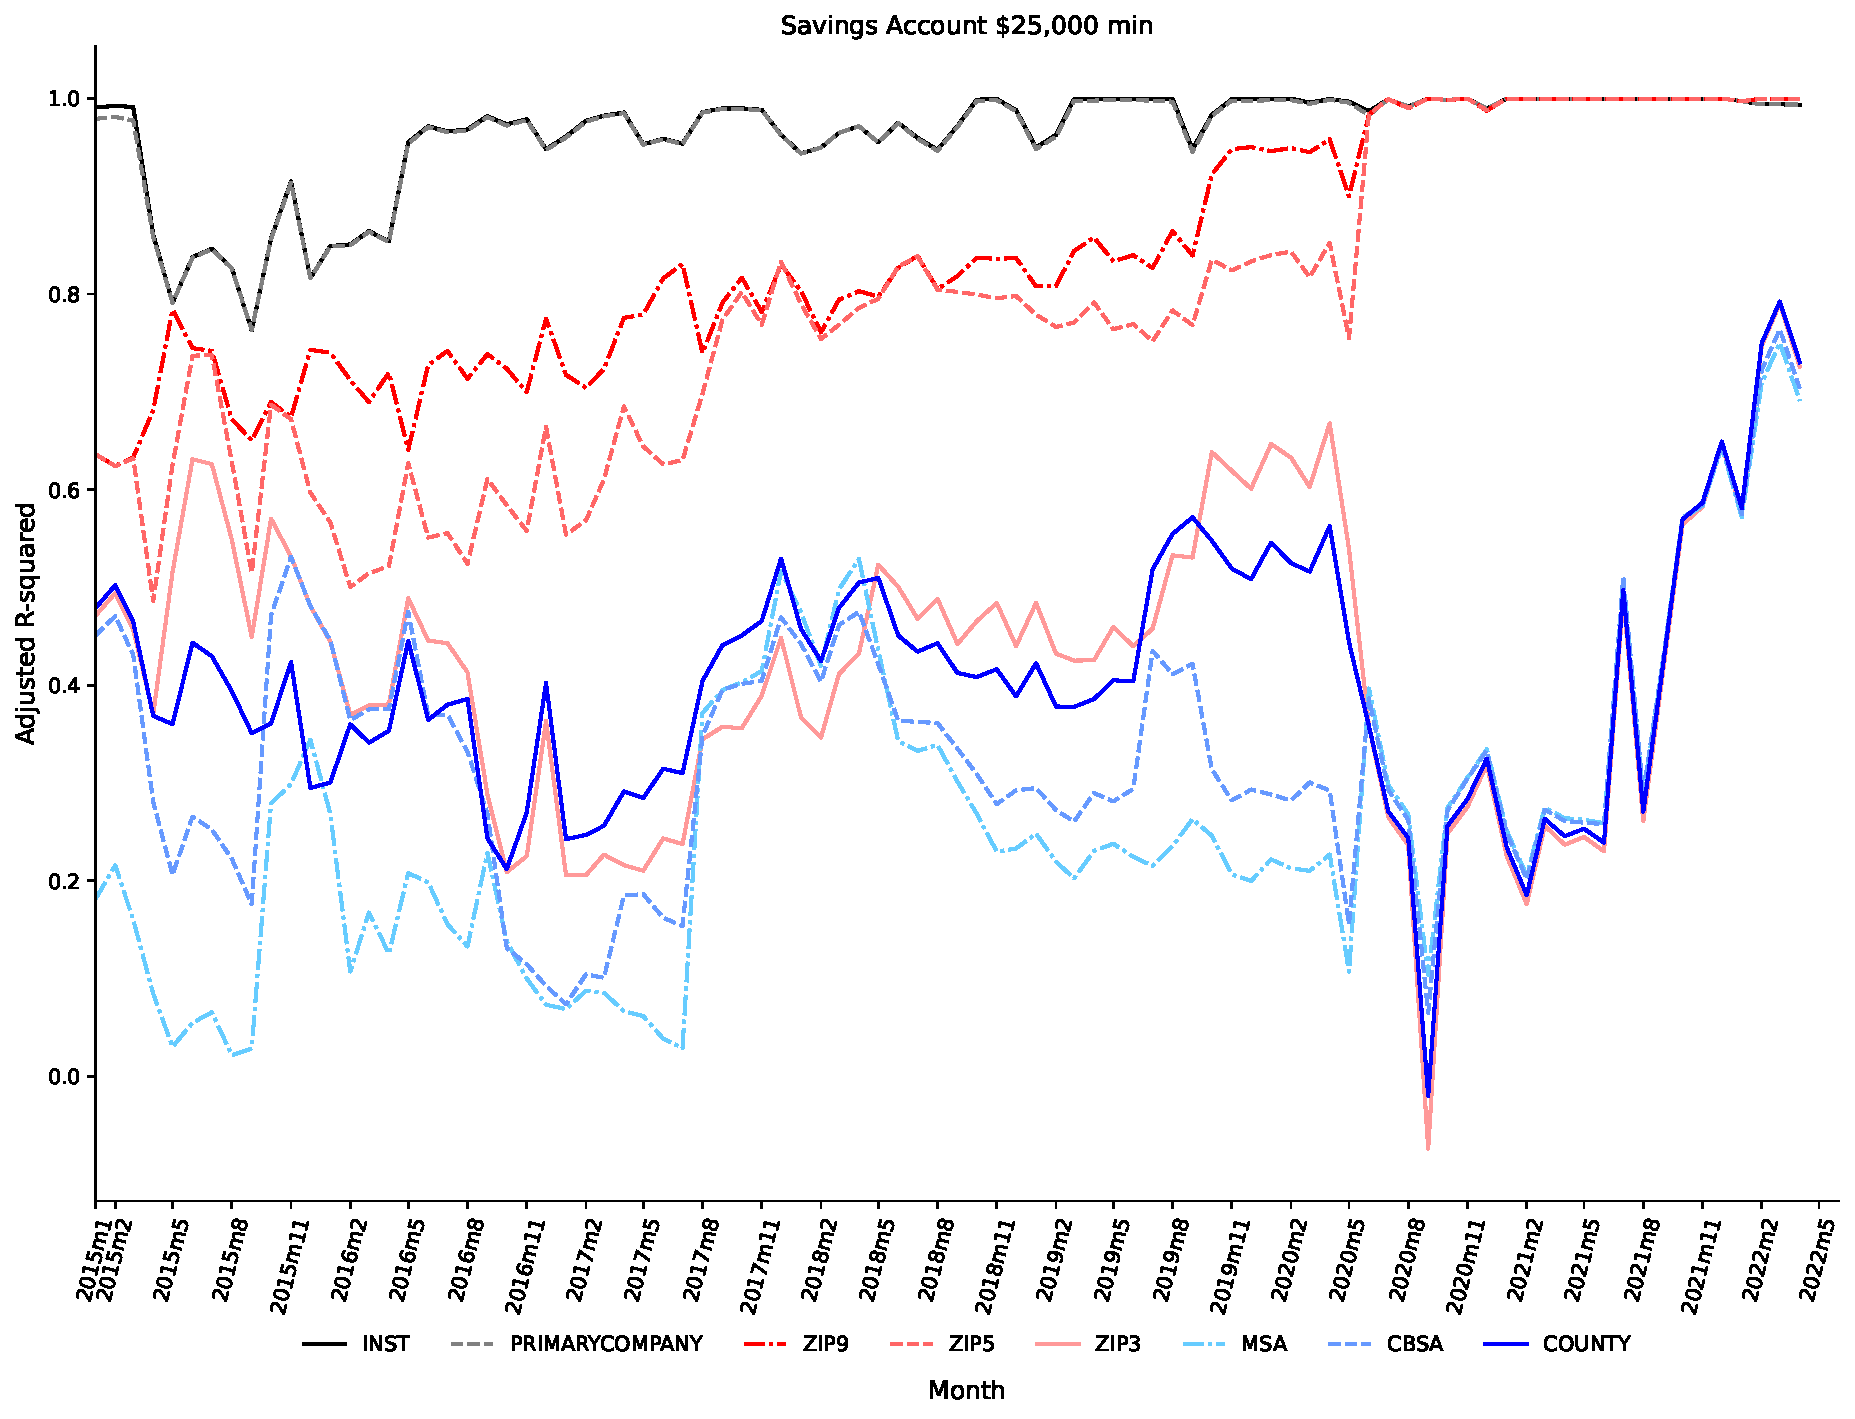
\includegraphics[width=1\textwidth]{figure/all_sample_939605/all_fixed_effects/SAV25K_adjusted_R2_all_fixed_effects.pdf} 
\end{center}
\end{frame}






\section{Run Reg on the Multi-branches Sample}

\subsection{The 3 Fixed Effects Proxies (similar to GP wp)}

\begin{frame}
    \vfill
    \centering
    {\usebeamercolor[fg]{structure} Multi-branches sample, figures similar to GP wp,}
    
    \begin{enumerate}
        \item Showing adjusted $R^2$ of rate regress on the following fixed effects, 
            
            Bank (inst\_nm), Zip Code (3 digits), Banking Market (MSA)
        \item Regression on the full sample, {\textbf{\usebeamercolor[fg]{structure}excluding}} 'inst\_nm's that have only single 'accountnumber'
    \end{enumerate}
    \vfill
\end{frame}


\begin{frame}{12MCD0K, multi-branches sample}
\begin{center}
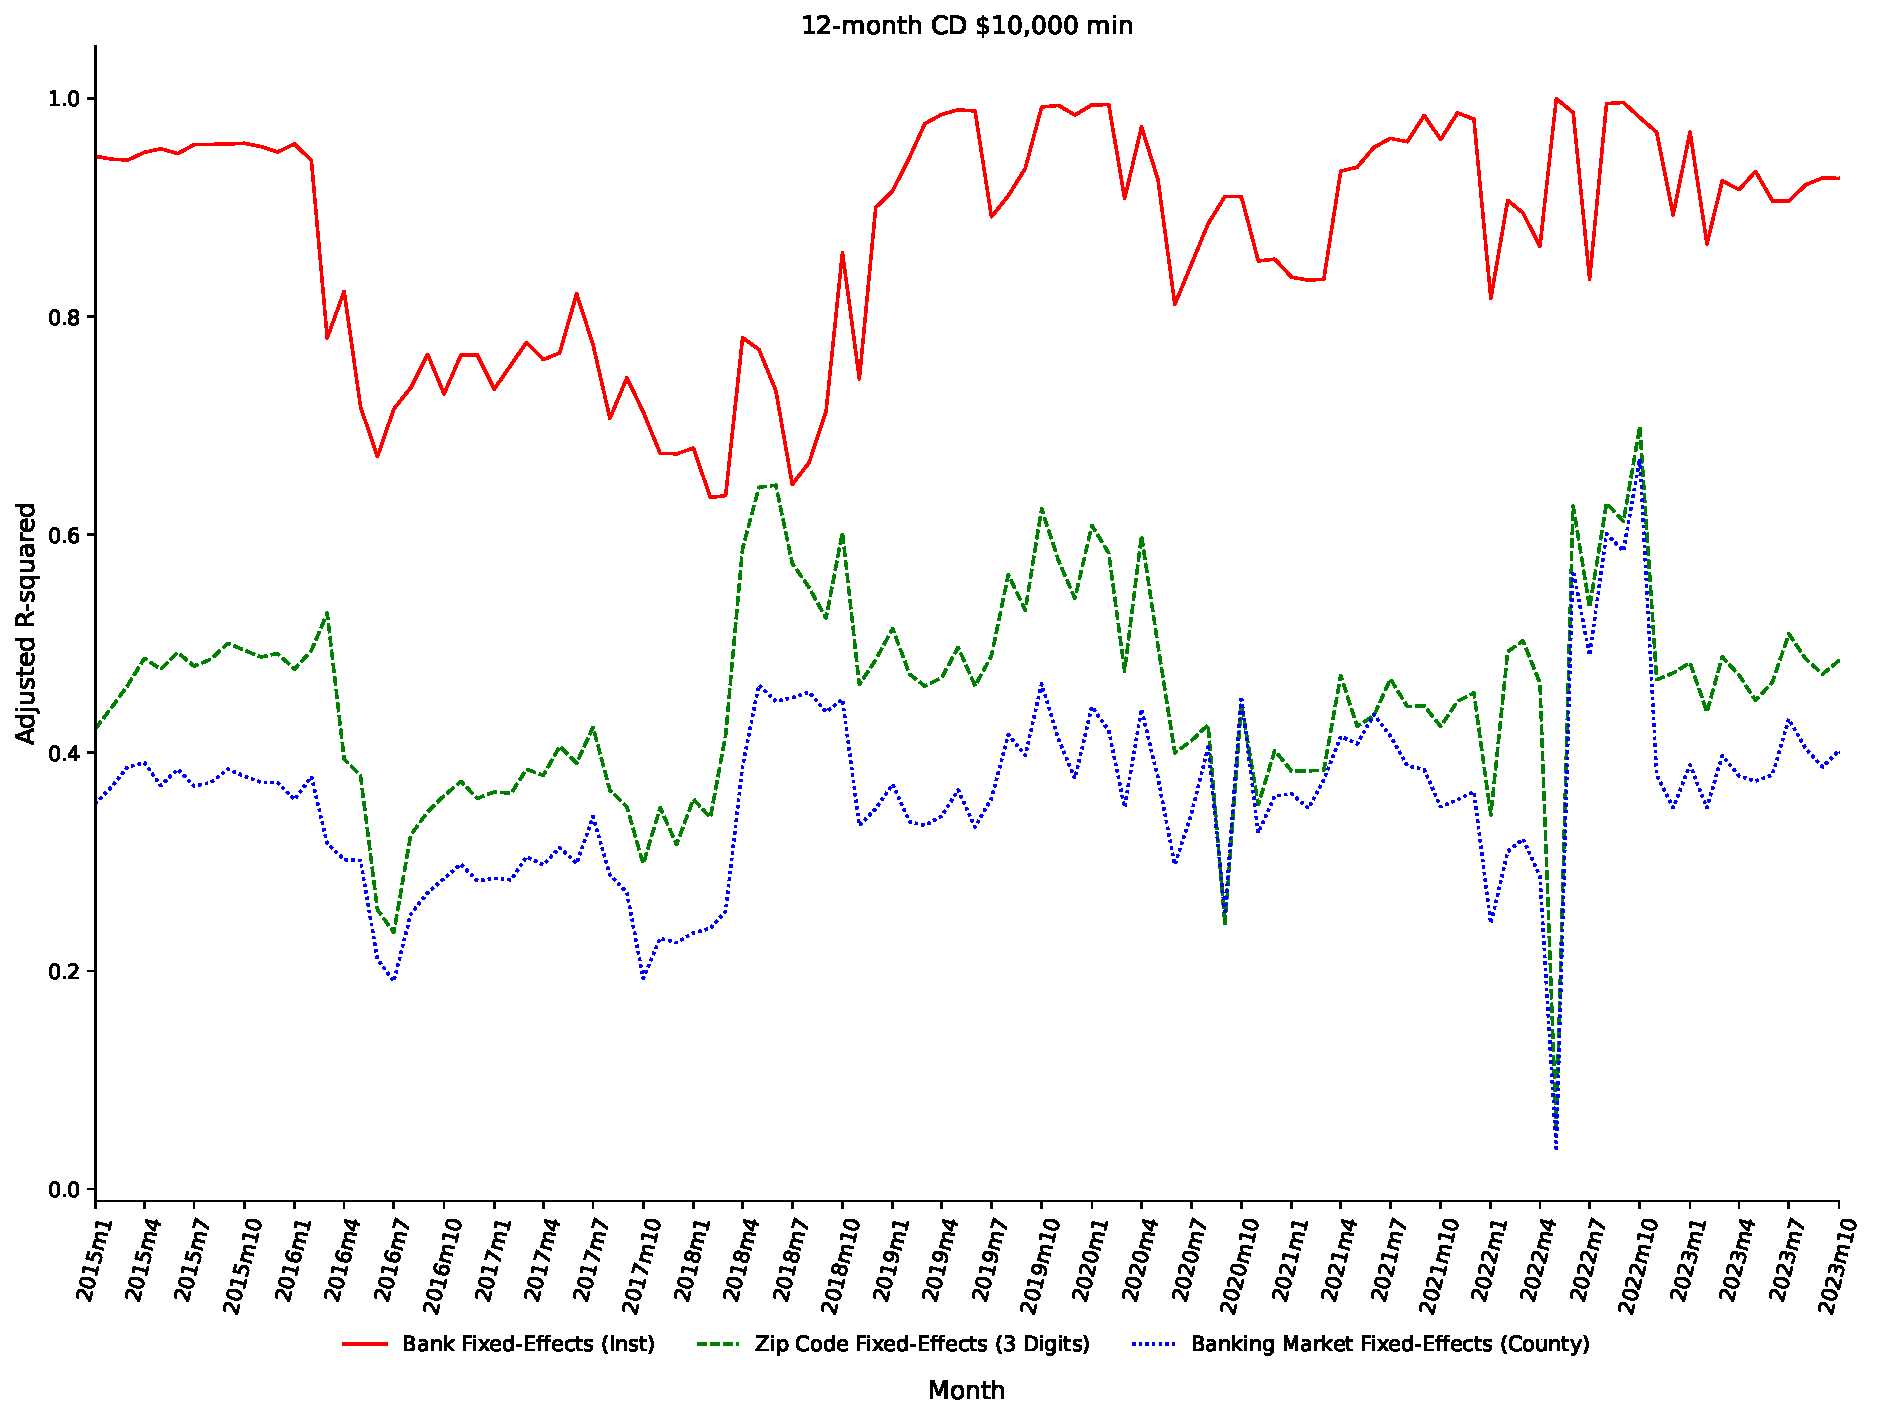
\includegraphics[width=1\textwidth]{figure/multi_branch_sample_932466/3_fixed_effects_same_as_GP_wp/12MCD10K_adjusted_R2_Rate_3_fixed_effects.pdf} 
\end{center}
\end{frame}


\begin{frame}{INTCK2.5K, multi-branches sample}
\begin{center}
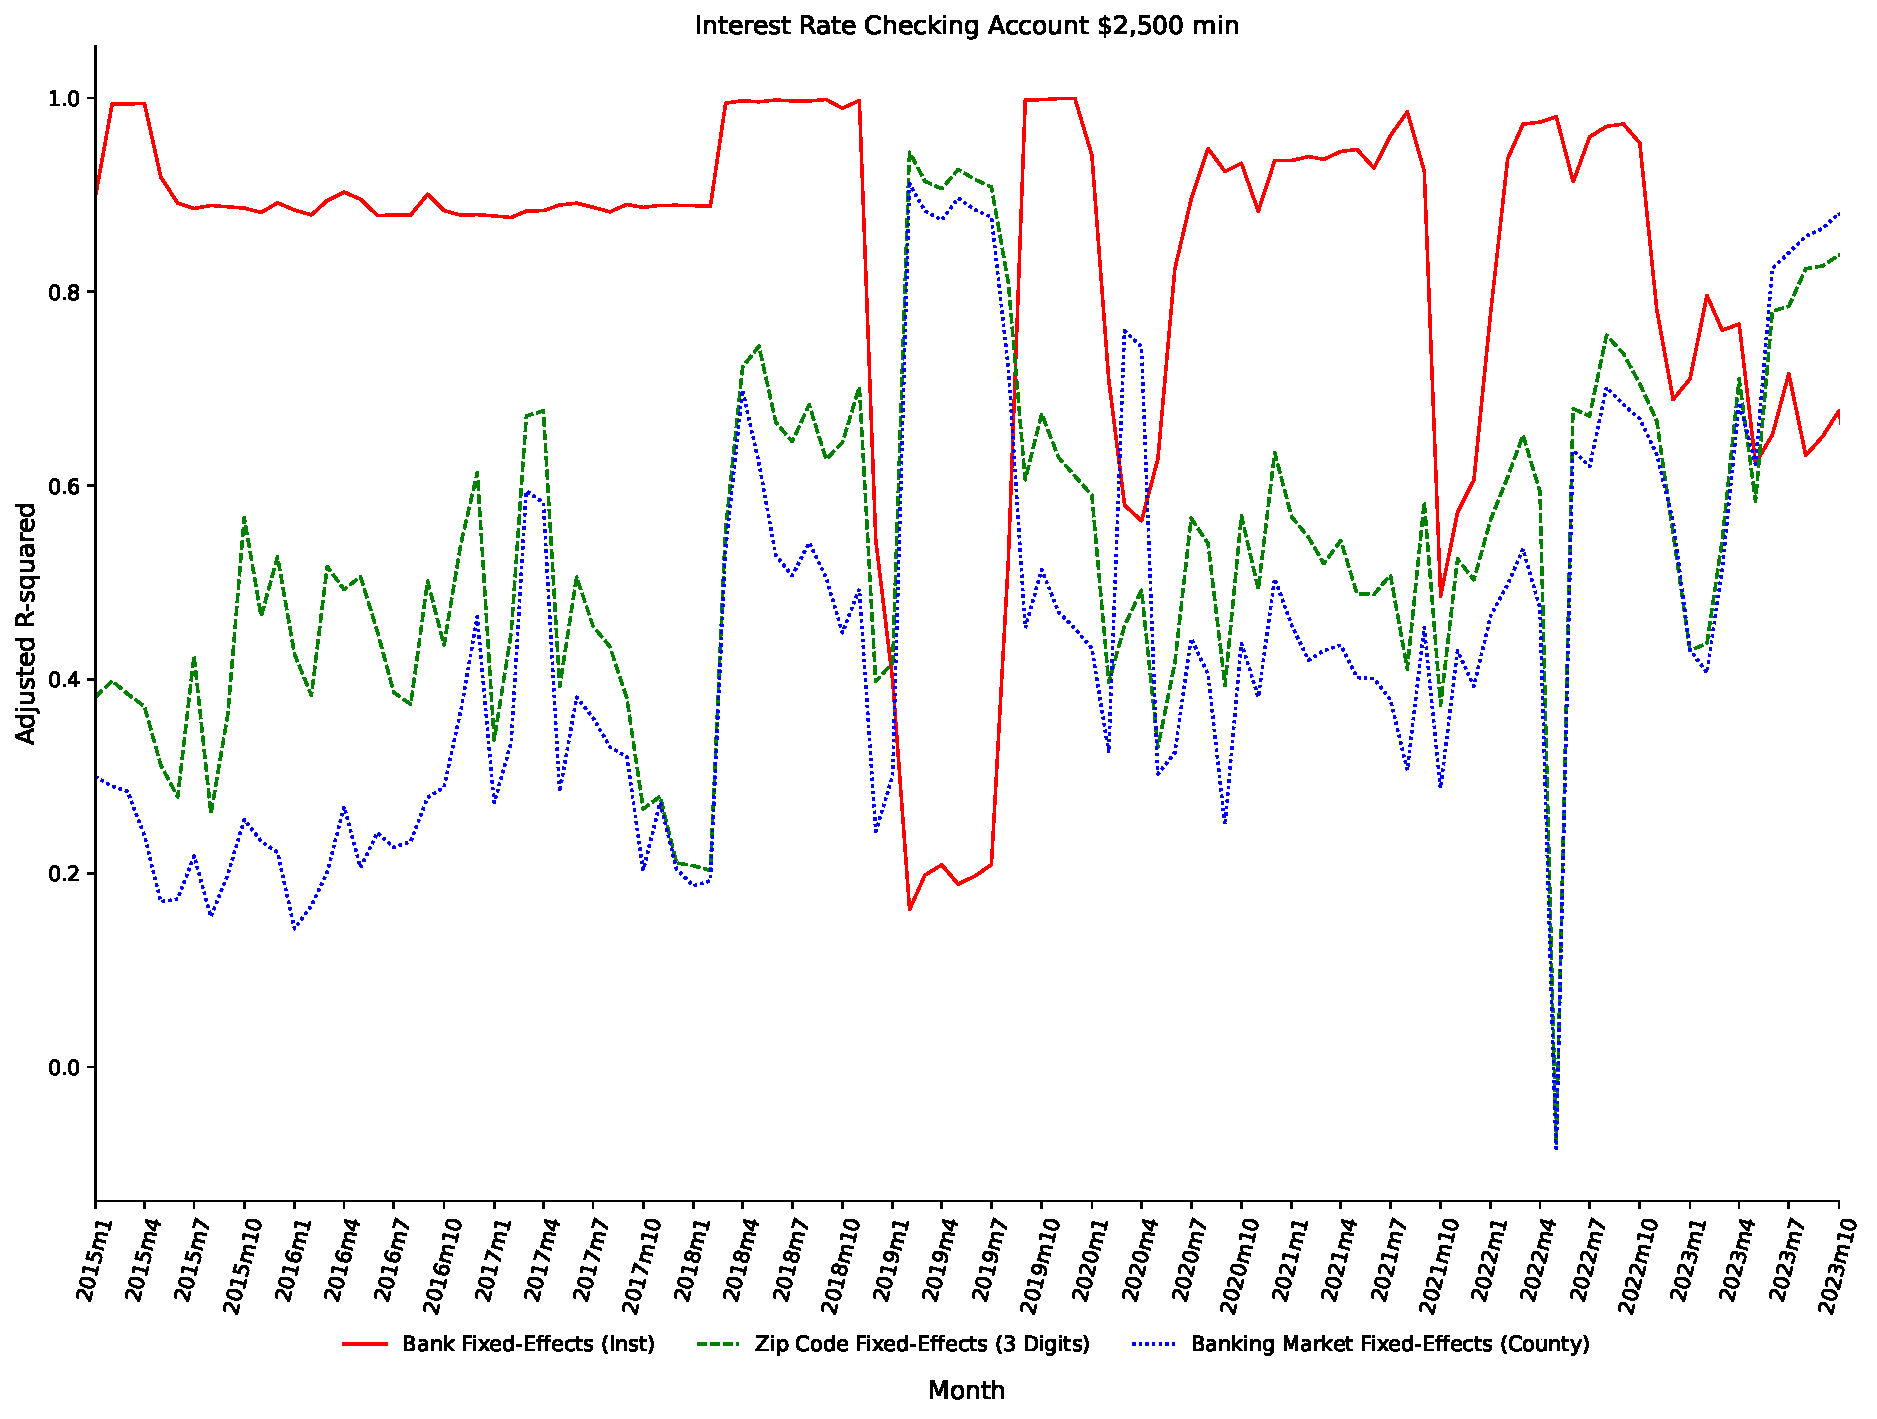
\includegraphics[width=1\textwidth]{figure/multi_branch_sample_932466/3_fixed_effects_same_as_GP_wp/INTCK2_5K_adjusted_R2_Rate_3_fixed_effects.pdf} 
\end{center}
\end{frame}



\begin{frame}{SAV2.5K, multi-branches sample}
\begin{center}
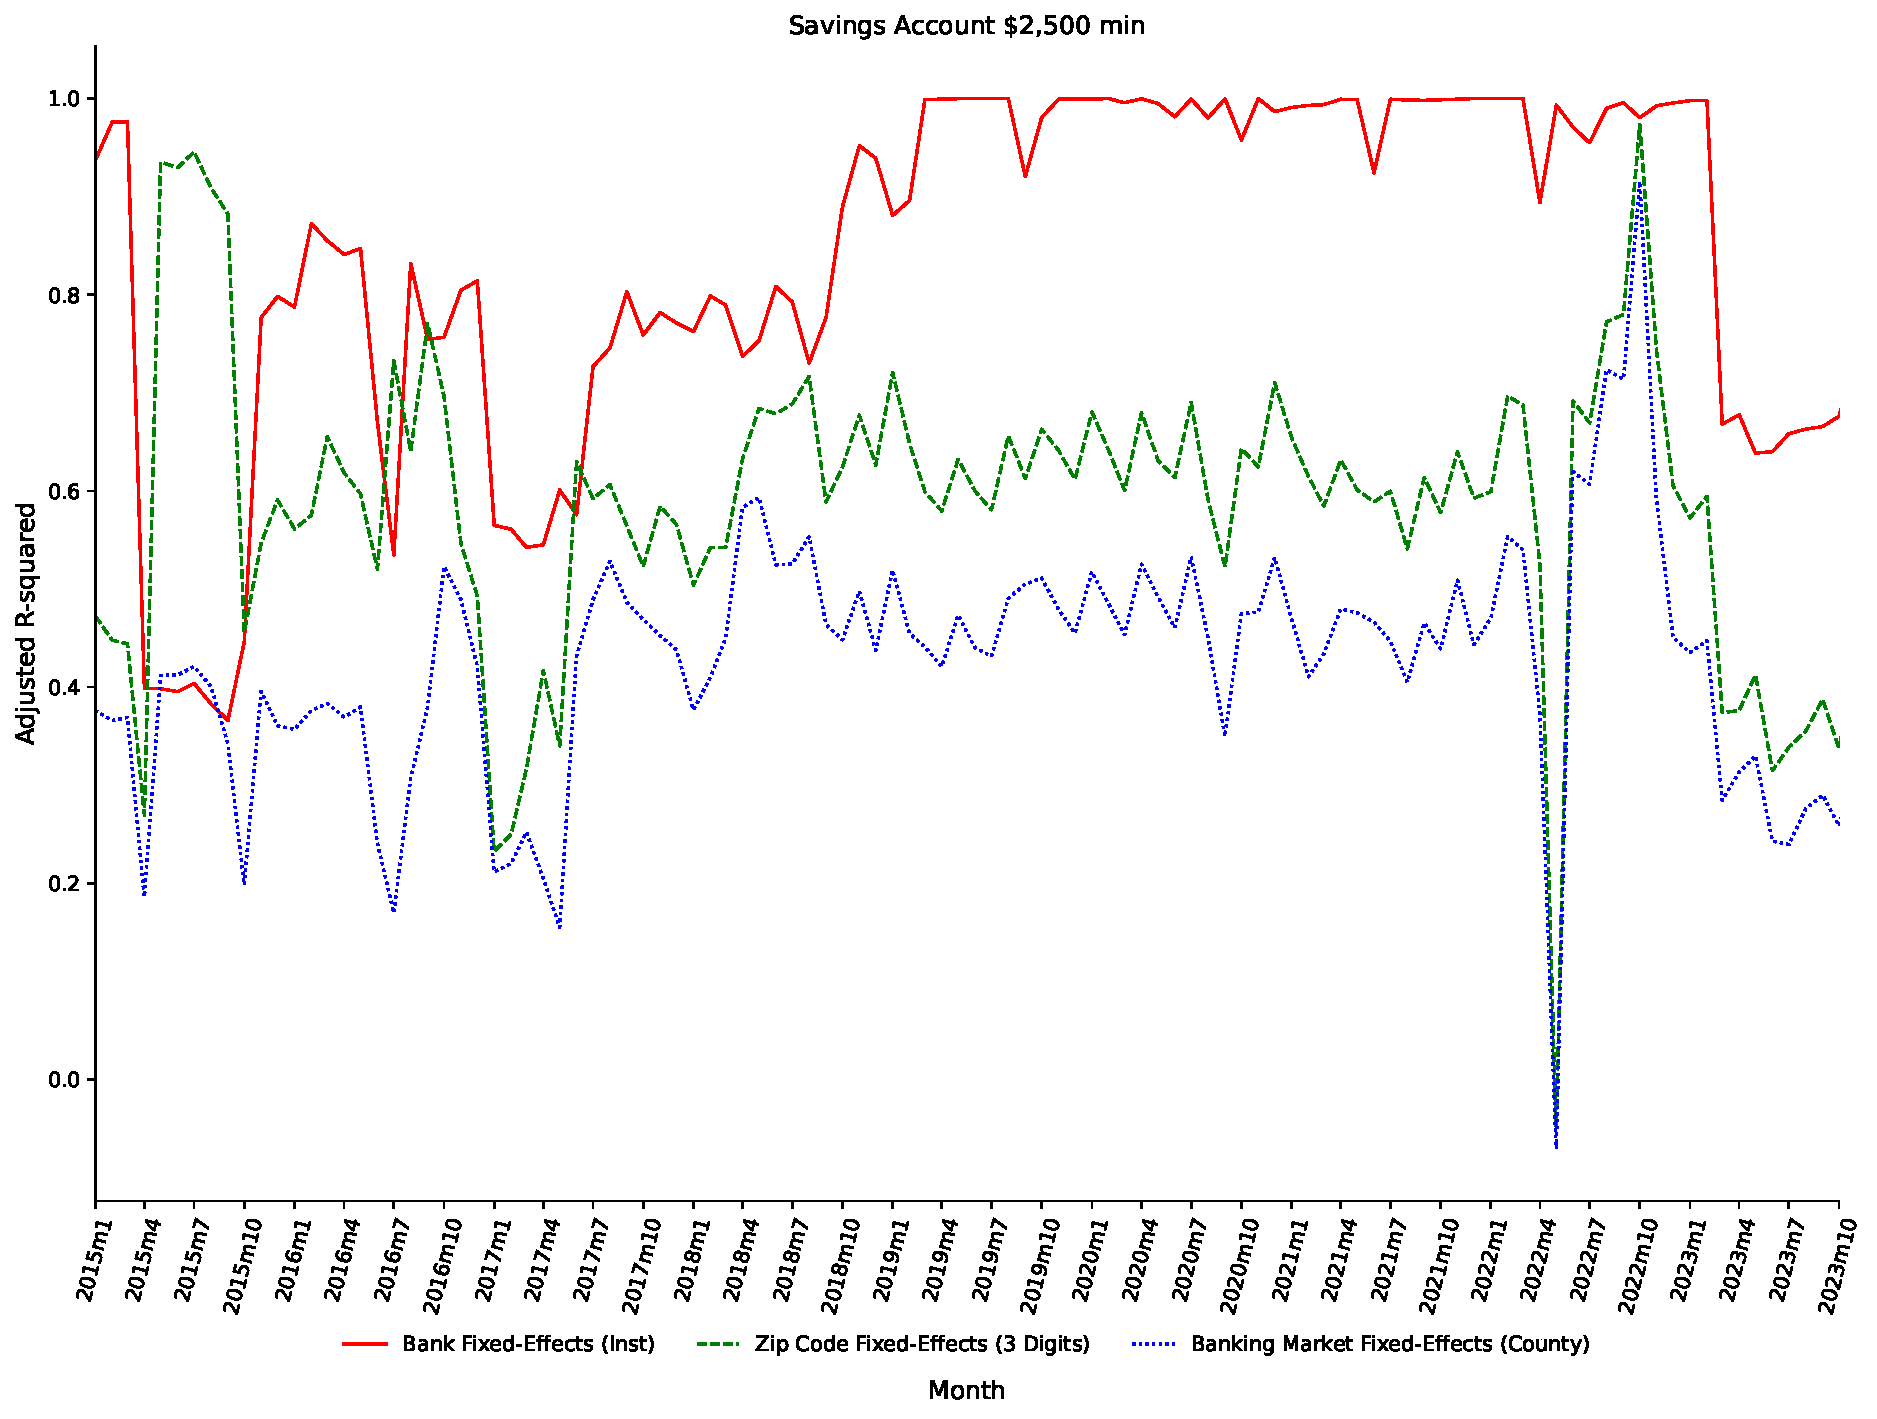
\includegraphics[width=1\textwidth]{figure/multi_branch_sample_932466/3_fixed_effects_same_as_GP_wp/SAV2_5K_adjusted_R2_Rate_3_fixed_effects.pdf} 
\end{center}
\end{frame}



\begin{frame}{SAV25K, multi-branches sample}
\begin{center}
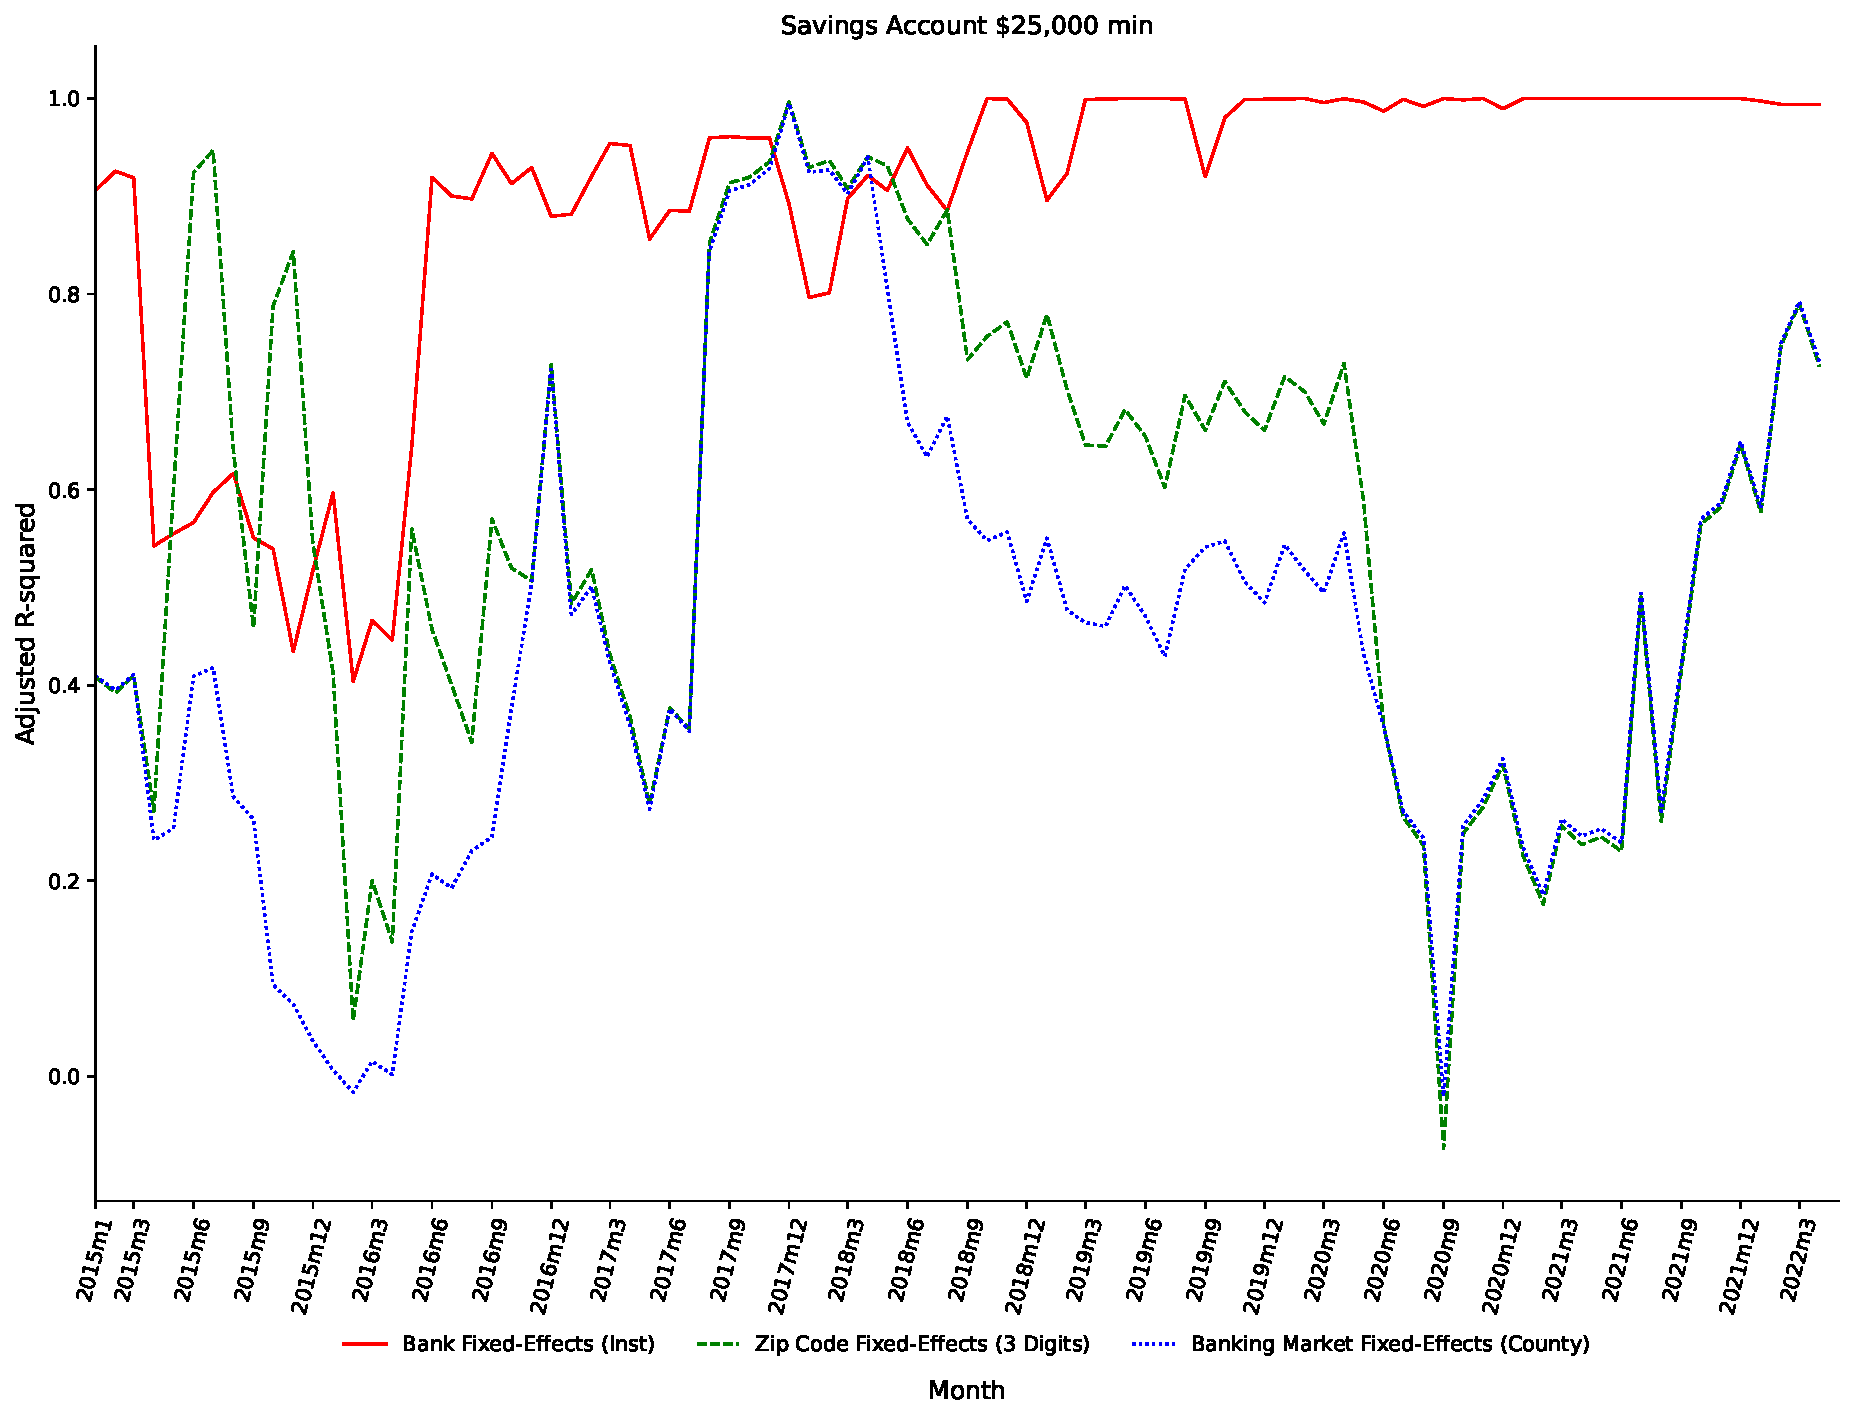
\includegraphics[width=1\textwidth]{figure/multi_branch_sample_932466/3_fixed_effects_same_as_GP_wp/SAV25K_adjusted_R2_Rate_3_fixed_effects.pdf} 
\end{center}
\end{frame}





\subsection{Comparison of all fixed effects proxies}

\begin{frame}
    \vfill
    \centering
    {\usebeamercolor[fg]{structure}Multi-branches sample, figures comparing all possible proxies,}
    \begin{enumerate}
        \item Showing adjusted $R^2$ of rate regress on fixed effects, using the following proxies, 
        \begin{itemize}
            \item Bank fixed effects: 'primarycompany' and 'inst\_nm
            \item Banking market fixed effects: 'msa' and 'cbsa'
            \item Zip code fixed effects: the first 3 or 5 or 9 digits of 'zip'
        \end{itemize}    
        \item Regression on the full sample, {\textbf{\usebeamercolor[fg]{structure}excluding}} 'inst\_nm's that have only single 'accountnumber'
    \end{enumerate}
    \vfill
\end{frame}


\begin{frame}{12MCD0K, multi-branches sample}
\begin{center}
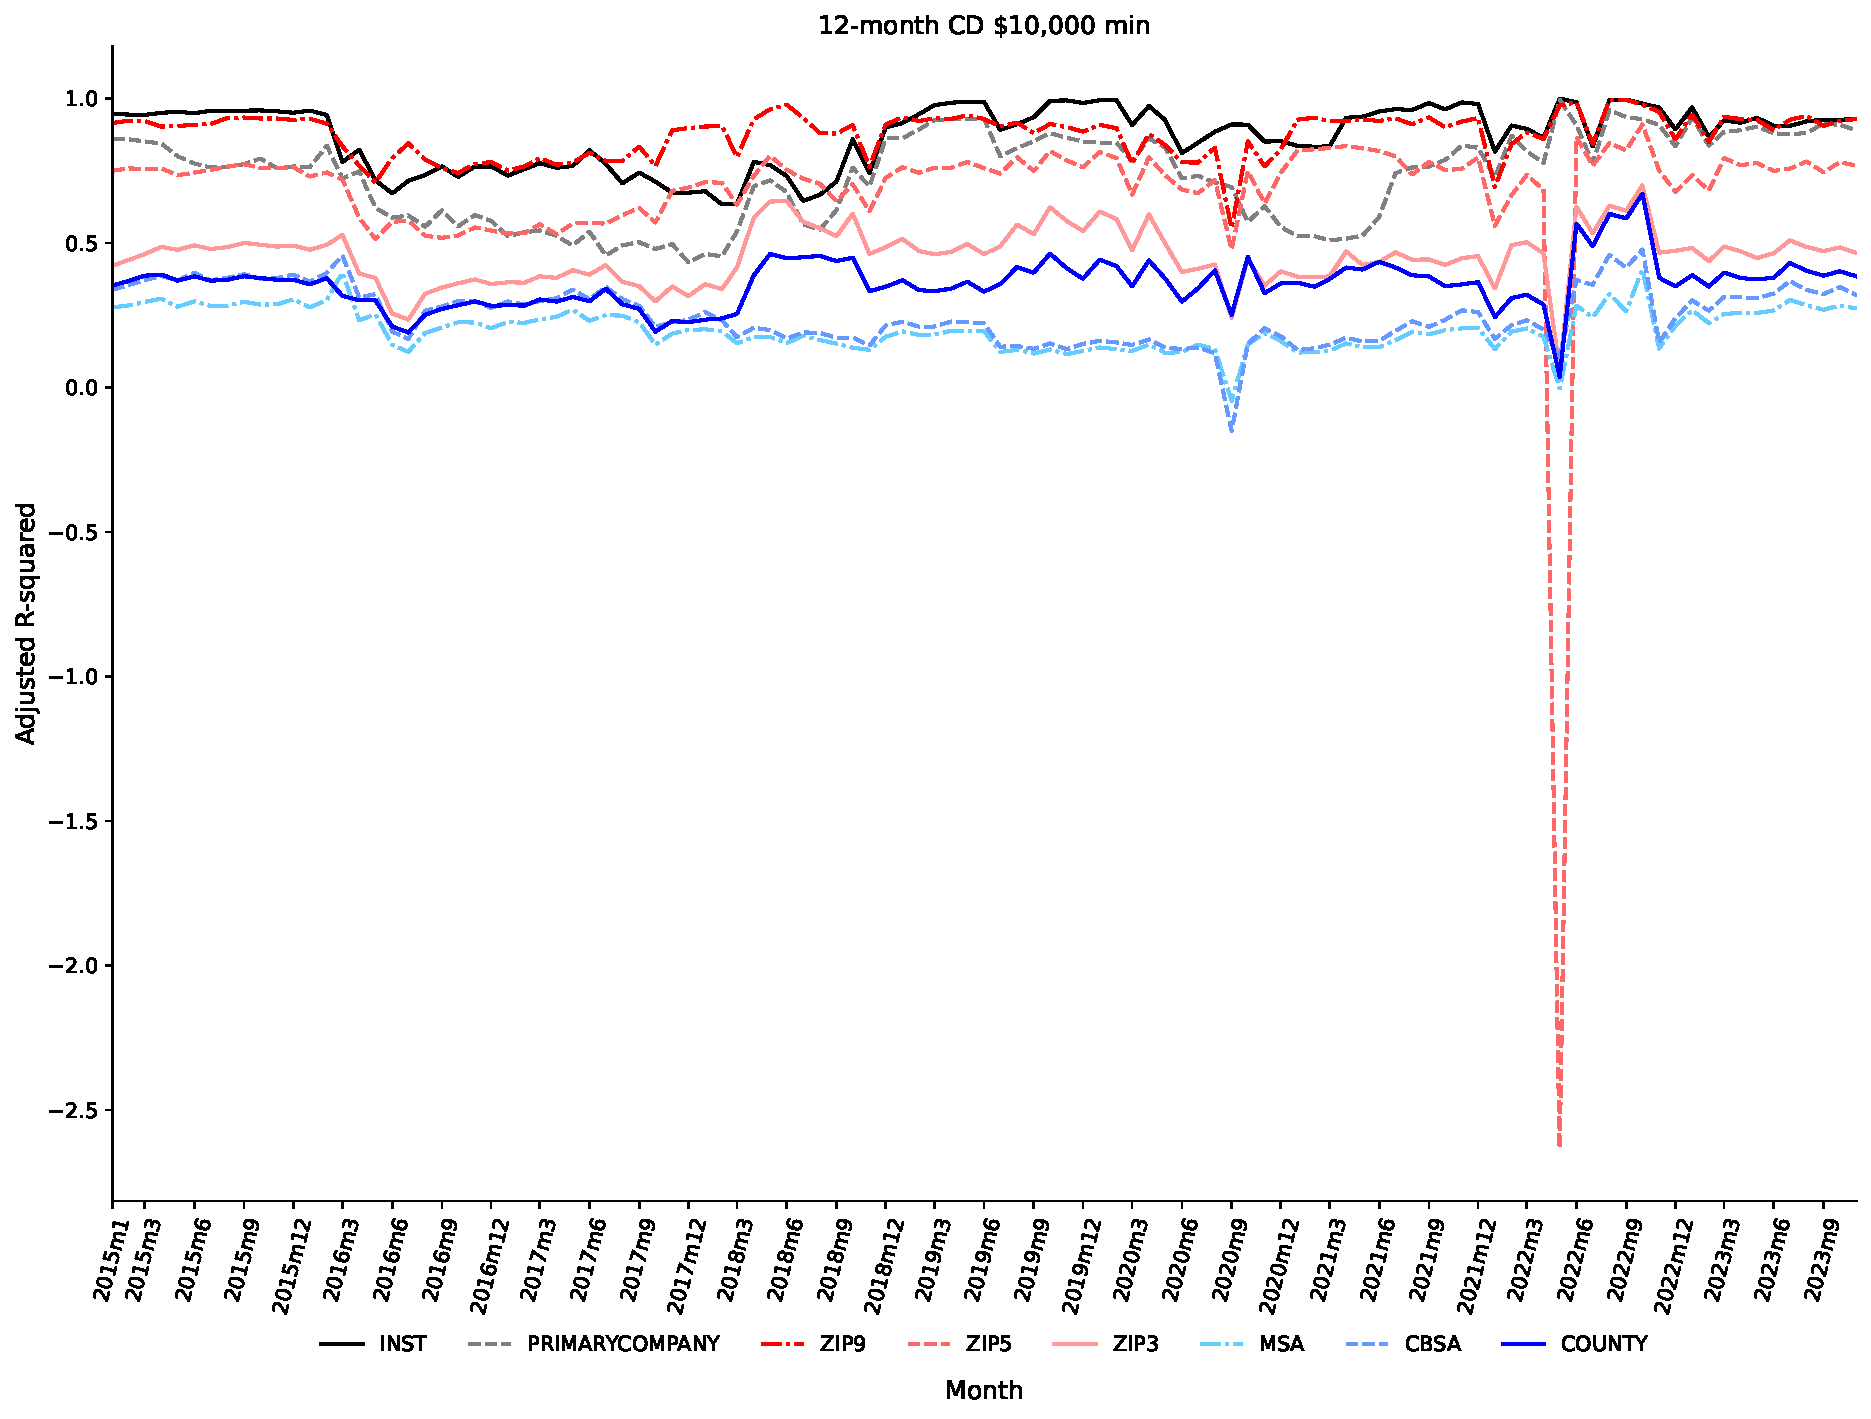
\includegraphics[width=1\textwidth]{figure/multi_branch_sample_932466/all_fixed_effects/12MCD10K_adjusted_R2_all_fixed_effects.pdf} 
\end{center}
\end{frame}


\begin{frame}{INTCK2.5K, multi-branches sample}
\begin{center}
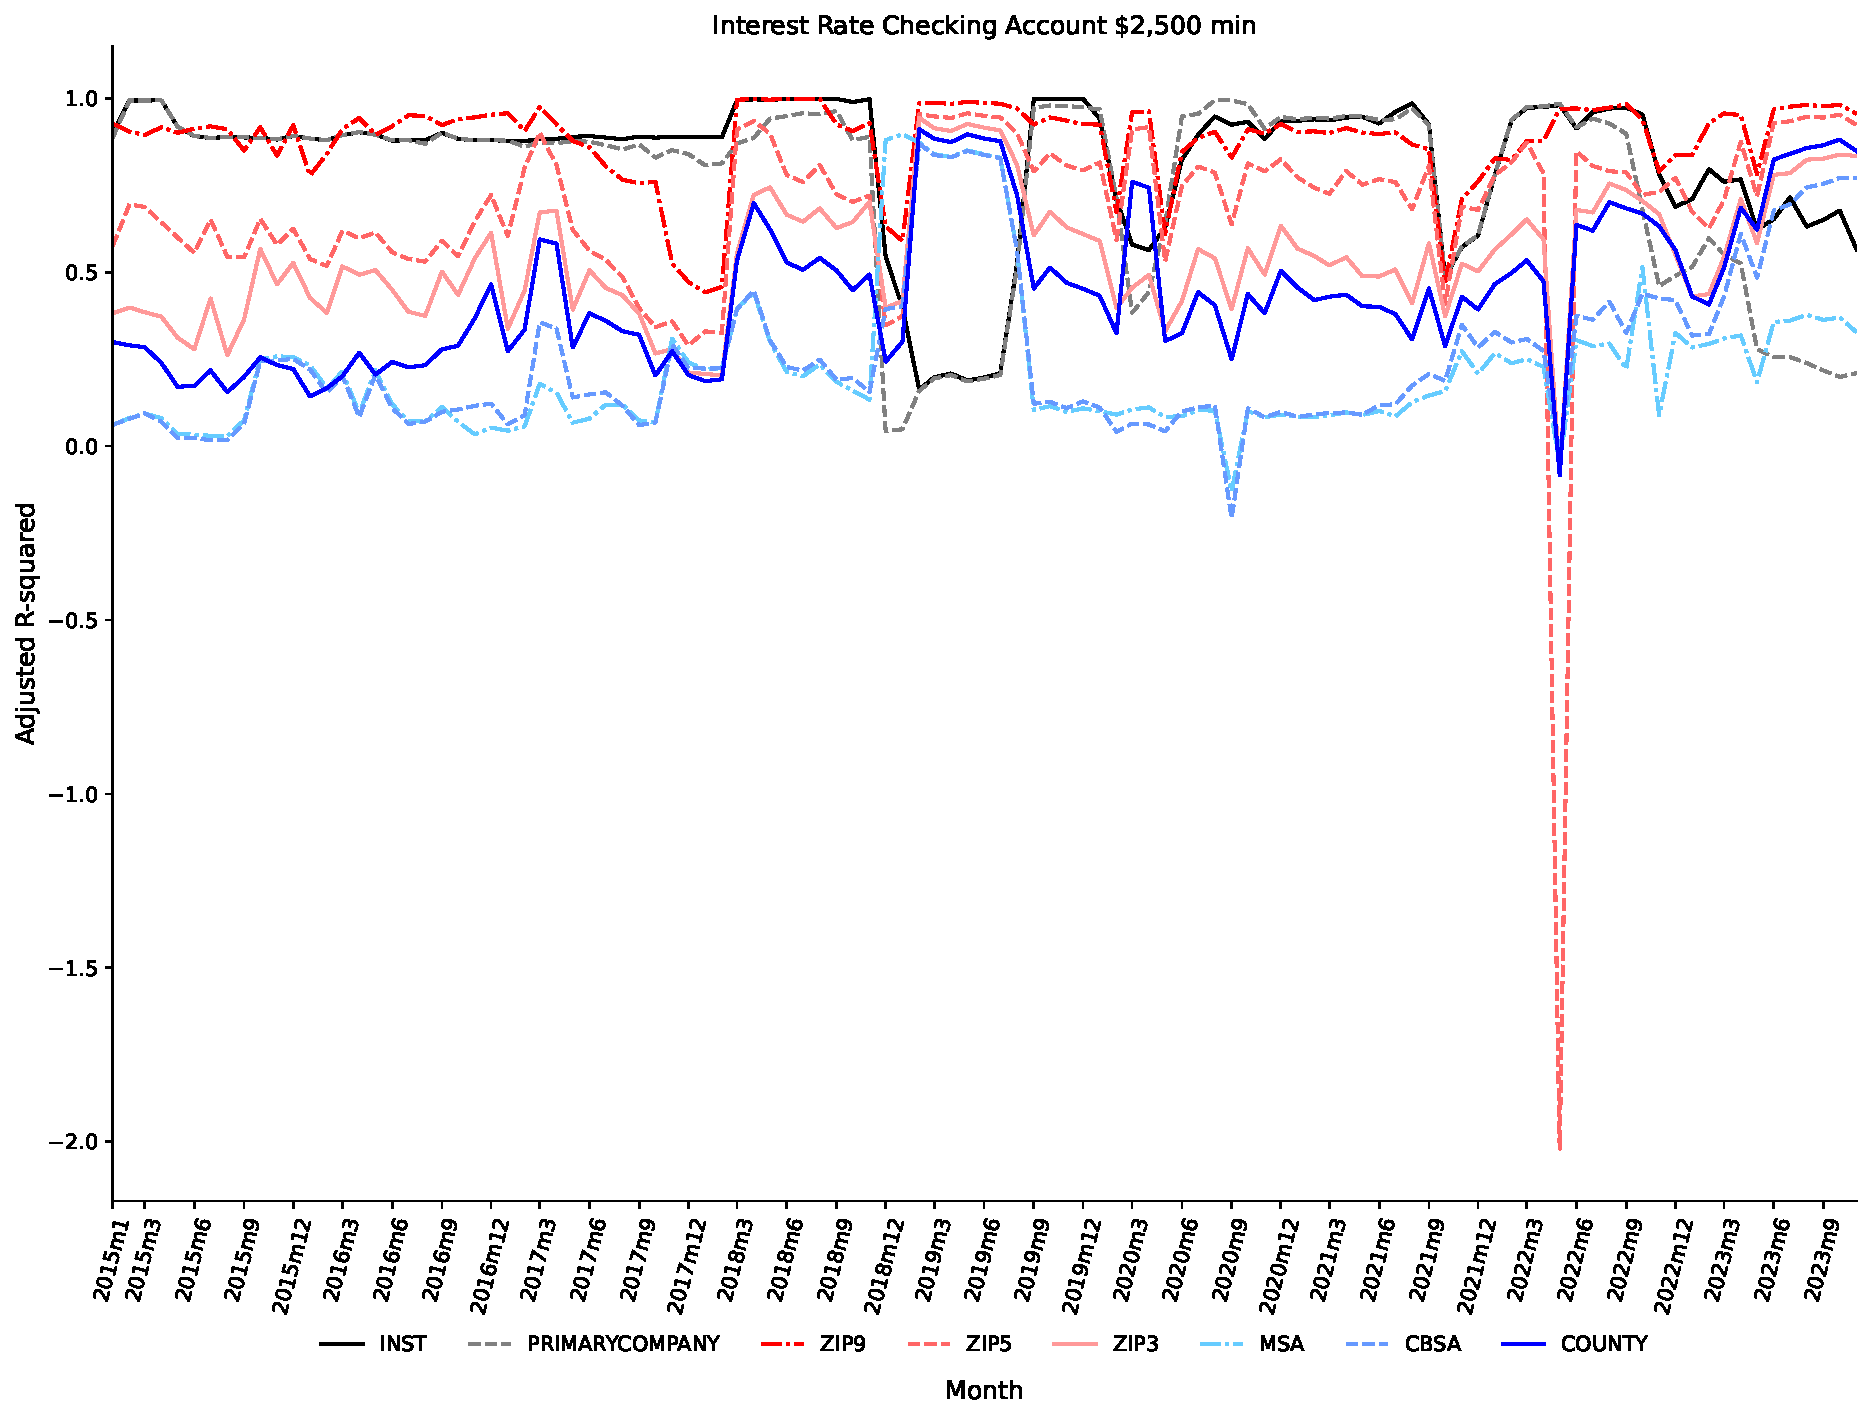
\includegraphics[width=1\textwidth]{figure/multi_branch_sample_932466/all_fixed_effects/INTCK2_5K_adjusted_R2_all_fixed_effects.pdf} 
\end{center}
\end{frame}



\begin{frame}{SAV2.5K, multi-branches sample}
\begin{center}
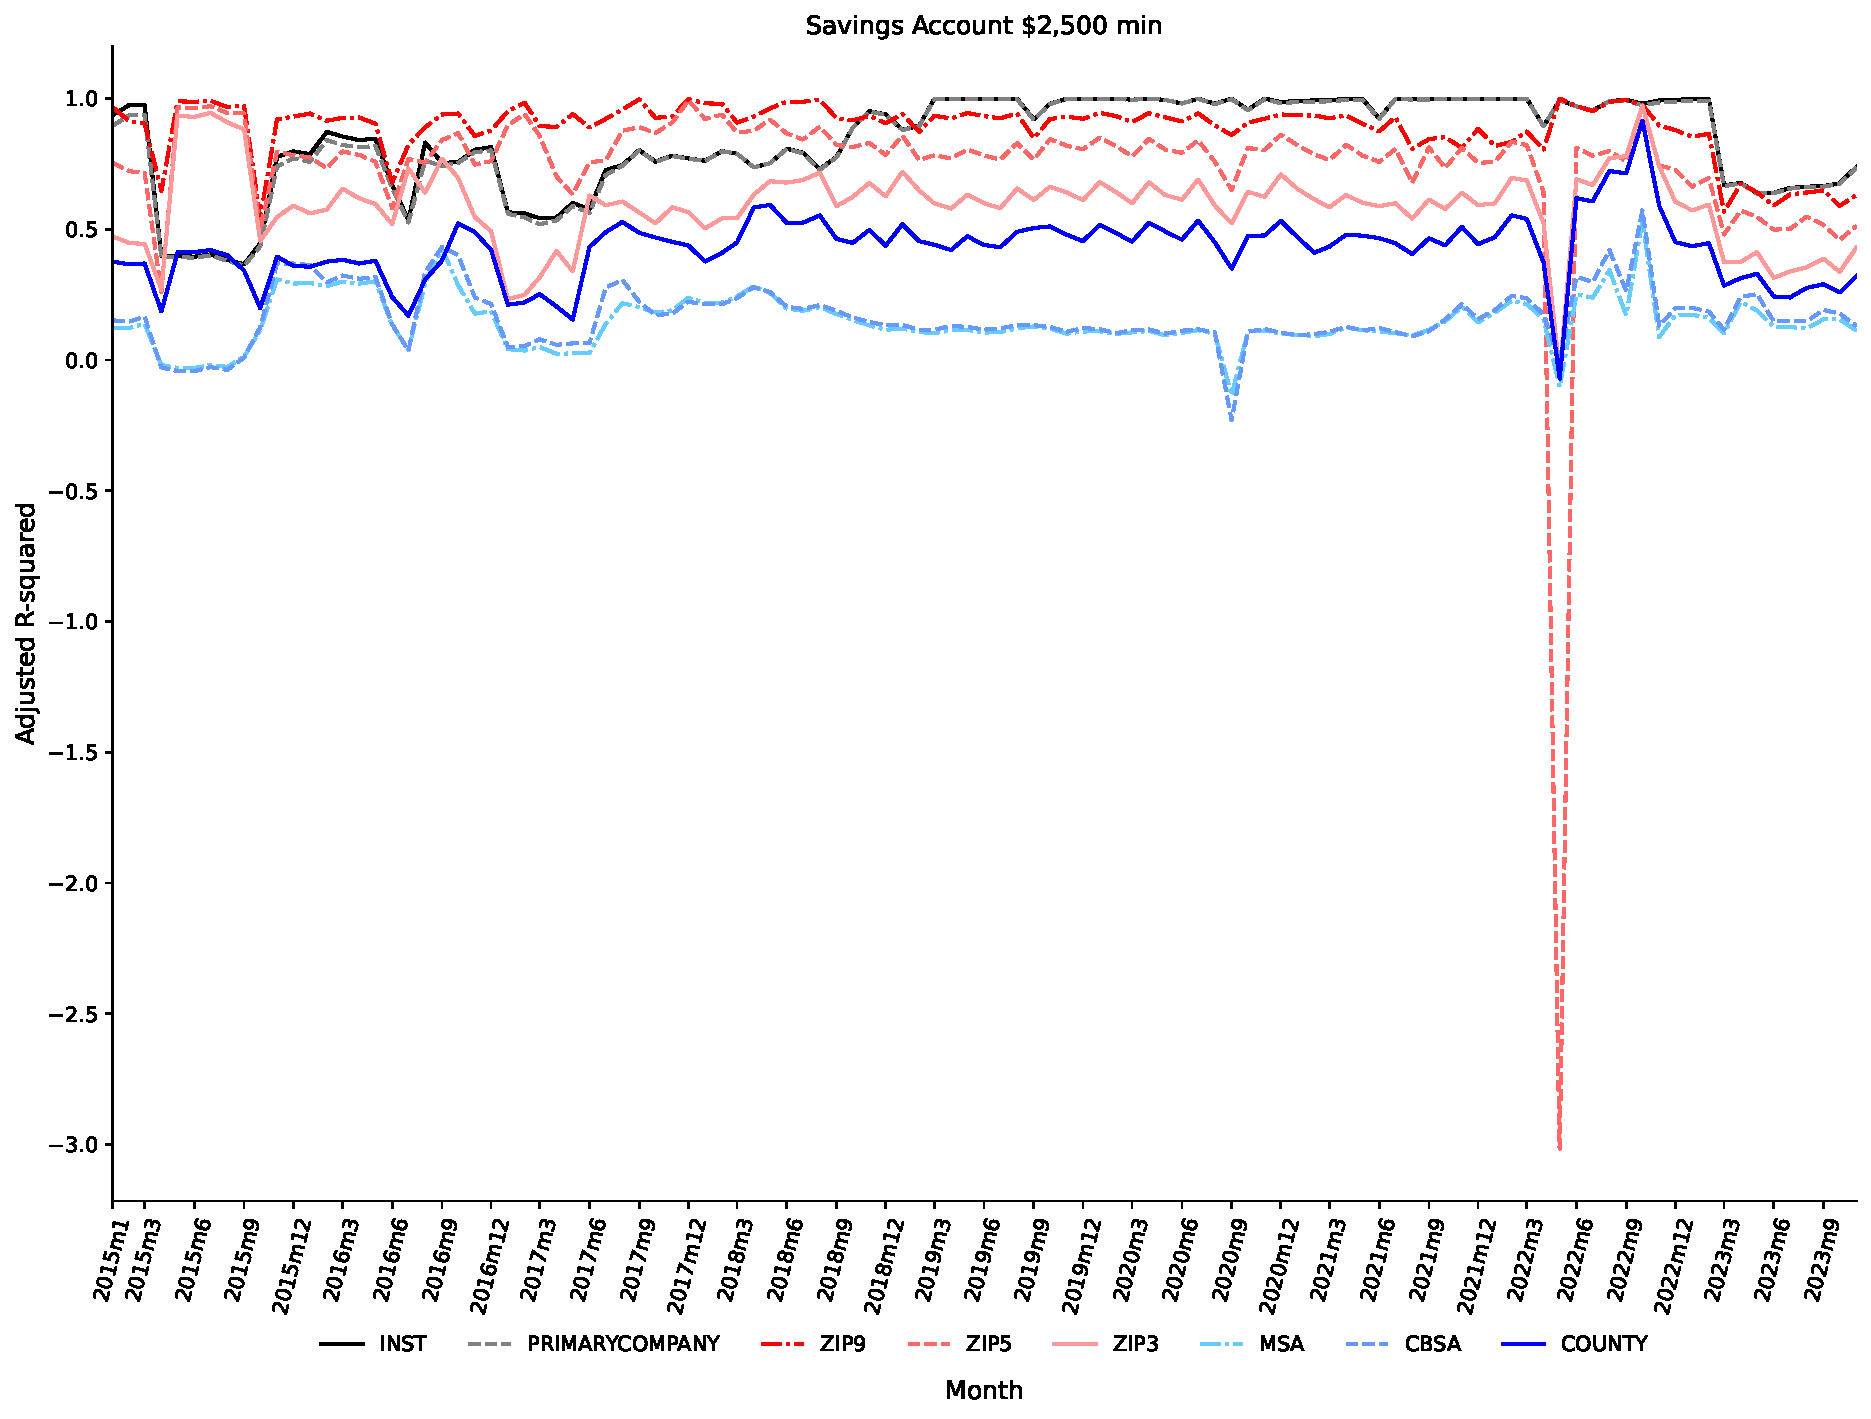
\includegraphics[width=1\textwidth]{figure/multi_branch_sample_932466/all_fixed_effects/SAV2_5K_adjusted_R2_all_fixed_effects.pdf} 
\end{center}
\end{frame}



\begin{frame}{SAV25K, multi-branches sample}
\begin{center}
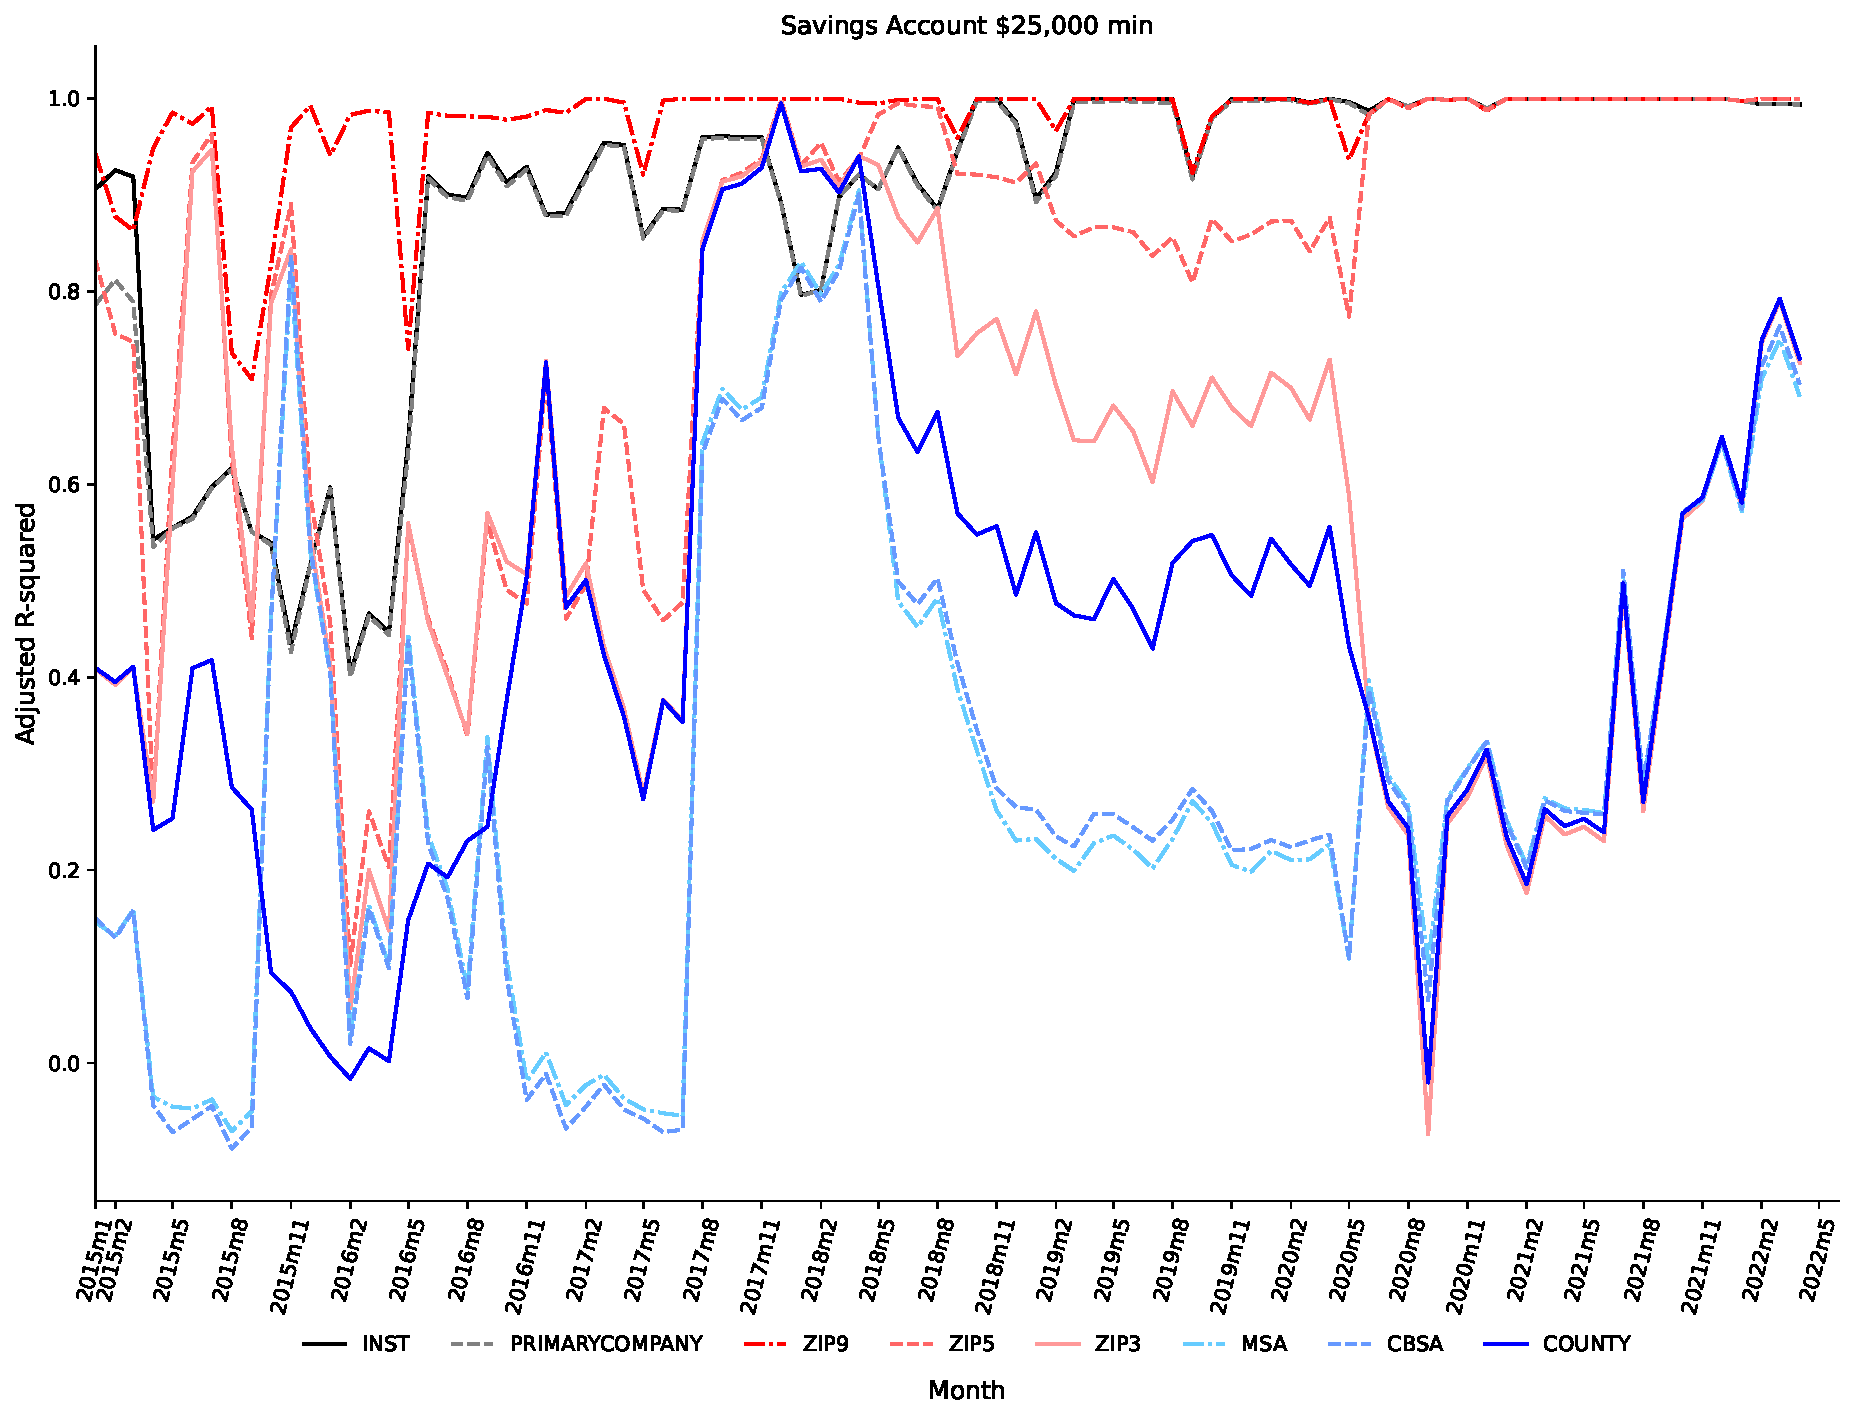
\includegraphics[width=1\textwidth]{figure/multi_branch_sample_932466/all_fixed_effects/SAV25K_adjusted_R2_all_fixed_effects.pdf} 
\end{center}
\end{frame}





\end{document}